\documentclass[aspectratio=169,11pt,t]{beamer}
% ============================================================
%  ksa-cs-v2: ksa-cs-lecture-template.tex 스타일 + 한글, v2 덱(16:9)용.
%    - 짙은 네이비 헤드라인 (섹션 이름 + 프레임마다 점)
%    - 꽉 찬 파란 제목 막대, 둥근 그림자 블록
%    - 한글: Noto Sans CJK KR (fontspec)
%  사용:
%    \documentclass[aspectratio=169,11pt,t]{beamer}
%    \input{<..>/theme/ksa-cs-v2.tex}
%  ksa-theme.tex 의 매크로(\kb \kq, ksablue/ksared 등)도 같은 이름으로 둔다
%  -> v2 덱 본문을 거의 그대로 옮길 수 있다.
% ============================================================

\usepackage{fontspec}
\usepackage{amsmath,amssymb}
\usepackage{tikz}
\usepackage{listings}
\usepackage{graphicx}
\usepackage{booktabs}
\usepackage{varwidth}
% enumitem 은 넣지 않는다 (beamer 글머리표가 사라진다)

\defaultfontfeatures{Ligatures=TeX}
\setmainfont{Noto Sans CJK KR}
\setsansfont{Noto Sans CJK KR}
\setmonofont{Noto Sans Mono CJK KR}[Scale=0.92]
\usefonttheme{professionalfonts}

% ---------- 기본 틀 ----------
\usetheme{default}
\useinnertheme[shadow=true]{rounded}
\setbeamertemplate{navigation symbols}{}
\setbeamersize{text margin left=1em,text margin right=1em}

% ---------- 색 (템플릿 원본 값) ----------
\definecolor{navydark}{HTML}{191959}
\definecolor{navydim}{HTML}{8888B0}
\definecolor{navytitle}{HTML}{262686}
\definecolor{navyblue}{HTML}{3333B2}
\definecolor{blockbodybg}{HTML}{E9E9F3}
\definecolor{examplegreen}{HTML}{006000}
\definecolor{examplebg}{HTML}{E5EFE5}
\definecolor{alertred}{HTML}{BF0000}
\definecolor{alertbg}{HTML}{F9E5E5}
% ksa-theme.tex 와 같은 이름 (본문 호환)
\colorlet{ksablue}{navytitle}
\colorlet{ksabluedk}{navydark}
\definecolor{ksagold}{HTML}{D6CBB1}
\definecolor{ksagolddk}{HTML}{A9976B}
\colorlet{ksared}{alertred}
\definecolor{ksagray}{HTML}{5B5B5B}

\setbeamercolor{structure}{fg=navyblue}
\setbeamercolor{alerted text}{fg=alertred}
\setbeamercolor{frametitle}{bg=navytitle,fg=white}
\setbeamercolor{title}{fg=white,bg=navytitle}
\setbeamercolor{block title}{bg=navytitle,fg=white}
\setbeamercolor{block body}{bg=blockbodybg,fg=black}
\setbeamercolor{block title example}{bg=examplegreen,fg=white}
\setbeamercolor{block body example}{bg=examplebg,fg=black}
\setbeamercolor{block title alerted}{bg=alertred,fg=white}
\setbeamercolor{block body alerted}{bg=alertbg,fg=black}
\setbeamercolor{item}{fg=navyblue}
\setbeamertemplate{itemize item}[circle]
\setbeamertemplate{itemize subitem}[triangle]

% ---------- 헤드라인: miniframes (섹션 이름 + 점) ----------
\useoutertheme[subsection=false]{miniframes}
\setbeamerfont{section in head/foot}{size=\tiny}
\setbeamercolor{section in head/foot}{bg=navydark,fg=white}
\setbeamercolor{mini frame}{fg=white}
\setbeamertemplate{mini frames}[circle]

% ---------- 제목 막대: 폭 꽉 채움, 두 줄까지 ----------
\setbeamerfont{frametitle}{size=\normalsize,series=\bfseries}
\setbeamertemplate{frametitle}{%
  \nointerlineskip
  \begin{beamercolorbox}[wd=\paperwidth,ht=2.7ex,dp=1.1ex,leftskip=.3cm,rightskip=.3cm]{frametitle}%
    \usebeamerfont{frametitle}\insertframetitle
  \end{beamercolorbox}}

% ---------- 쪽 번호: 오른쪽 아래 ----------
\setbeamertemplate{footline}{%
  \hfill
  {\color{navydim}\scriptsize\insertframenumber\,/\,\inserttotalframenumber}%
  \hspace{3mm}\vspace{2mm}%
}

% ---------- 표지: 템플릿처럼 헤드라인은 그대로, 가운데 둥근 그림자 상자에 제목 한 줄 ----------
% 덱에서:  {\setbeamertemplate{footline}{}\begin{frame}[c,noframenumbering]\titlepage\end{frame}}
\setbeamercolor{title}{fg=white,bg=navyblue}
\makeatletter
\setbeamertemplate{title page}{%
  \vfill
  \centering
  \begin{minipage}{0.84\paperwidth}
  \begin{beamercolorbox}[wd=\linewidth,sep=7pt,center,rounded=true,shadow=true]{title}
    {\usebeamerfont{title}\inserttitle\par}%
    \ifx\insertsubtitle\@empty\else\vskip0.4em{\usebeamerfont{subtitle}\insertsubtitle\par}\fi
  \end{beamercolorbox}
  \end{minipage}\par\vskip1.6em
  {\usebeamerfont{author}\color{navytitle}\insertauthor\par}\ifx\beamer@date\@empty\vskip0.3em\else\vskip1.3em\fi
  {\usebeamerfont{institute}\color{ksagray}\insertinstitute\par}%
  \ifx\beamer@date\@empty\else\vskip0.3em{\usebeamerfont{date}\color{ksagray}\insertdate\par}\fi
  \vfill
}
\makeatother
\setbeamerfont{title}{series=\bfseries,size=\Large}
\setbeamerfont{subtitle}{size=\normalsize}
\setbeamerfont{author}{size=\normalsize}
\setbeamerfont{institute}{size=\small}
\setbeamerfont{date}{size=\small}

% ksa-theme 호환: 덱이 \renewcommand{\ksacredit}{..} 를 해도 되게 (꼬리말에는 안 쓴다)
\newcommand{\ksacredit}{}

% ---------- 강조 ----------
\newcommand{\hl}[1]{\textcolor{alertred}{#1}}
\newcommand{\hlb}[1]{\textcolor{navyblue}{#1}}
\newcommand{\kb}[1]{\textbf{\color{ksablue}#1}}
\newcommand{\kq}[1]{\textbf{\color{ksared}#1}}

% ---------- 파이썬 코드 (템플릿과 같은 색) ----------
\definecolor{codekw}{HTML}{0033B3}
\definecolor{codebuiltin}{HTML}{BF0000}
\definecolor{codestr}{HTML}{067D17}
\definecolor{codecomment}{HTML}{8C8C8C}
\definecolor{codenum}{HTML}{1750EB}
\lstdefinestyle{py}{
  language=Python, basicstyle=\ttfamily\scriptsize,
  keywordstyle=\color{codekw}\bfseries, stringstyle=\color{codestr},
  commentstyle=\color{codecomment}\itshape, numberstyle=\color{codenum},
  emph={print,len,range,sum,input,int,str,float,list,dict,append,remove,sorted,abs,min,max},
  emphstyle=\color{codebuiltin}, showstringspaces=false, keepspaces=true,
  columns=fixed, basewidth=0.52em, aboveskip=1mm, belowskip=1mm, xleftmargin=2mm,
  breaklines=true
}
\lstset{style=py}

% SVM 덱(../2_svm)의 커널 부분을 나눠 만든 2차시 덱 (2026-11-21). 그림 원본 make_figs.py, 숫자 data.py
\setbeamerfont{author}{size=\normalsize}
\setbeamerfont{institute}{size=\small}
\graphicspath{{figs/}{../../../assets/}}
\usetikzlibrary{tikzmark,shapes.callouts,positioning}
\tikzset{bub/.style={draw=ksagolddk,line width=1pt,fill=ksagolddk!10,rounded corners=3pt,inner sep=4pt,font=\normalsize,align=left},
         bubarr/.style={-latex,ksagolddk,line width=1.2pt}}
\definecolor{fx}{HTML}{D62728}\definecolor{fsh}{HTML}{2E3192}\definecolor{fbeta}{HTML}{7A6A3F}\definecolor{fdist}{HTML}{2B8A3E}\definecolor{fbd}{HTML}{555555}
\makeatletter
\newcommand{\markpage}[1]{\protected@write\@auxout{}{\string\newlabel{#1}{{\the\c@framenumber}{}}}\hypertarget{#1}{}}
\newcommand{\pref}[1]{\hyperlink{#1}{\textcolor{ksagolddk}{(p.\ref{#1})}}}
\makeatother

\renewcommand{\ksacredit}{Machine Learning and Deep Learning \,\textperiodcentered\, 커널 SVM}
\title{커널 SVM (Kernel SVM)}
\subtitle{특징 늘리기 · 커널 트릭 · 다항 · RBF}
\author{Machine Learning and Deep Learning}
\institute{KSA 2027-Spring}
\date{Sumin Han (suminhan@ksa.hs.kr)}
\begin{document}
{\setbeamertemplate{footline}{}\begin{frame}[c,noframenumbering]\titlepage\end{frame}}

\section{질문}
% --- 지난 시간
\begin{frame}{지난 시간: 선형 SVM}
\vfill
\centering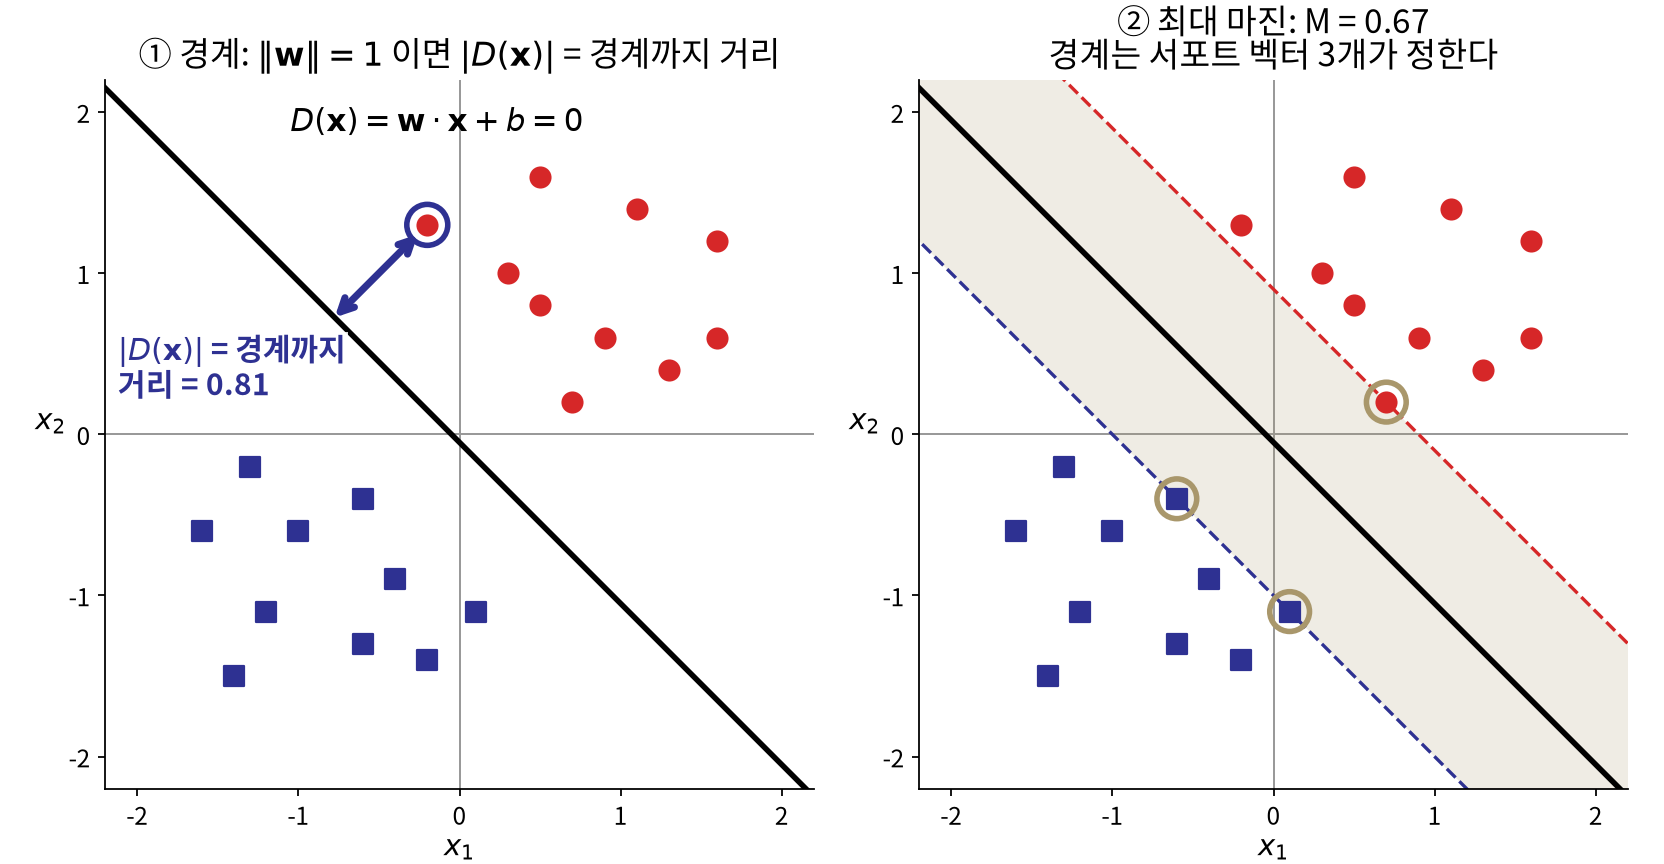
\includegraphics[width=0.96\linewidth]{kn_recap.png}\par\vskip0.2em
{\normalsize $C$ = 넘어간 양의 벌점, 크면 좁은 길}\\[0.4em]
{\Large 그런데 경계는 늘 \kq{직선}}
\vfill
\note{지난 시간 내용을 그림 세 장으로 정리합니다. 첫 번째 그림, 경계는 초평면 D x, w 점곱 x 더하기 b가 0인 곳이고, w의 길이를 1로 맞추면 점의 값이 곧 경계까지의 거리입니다. 그림의 파란 점은 값이 1.10, 경계까지 거리도 1.10입니다. 두 번째 그림, 가장 가까운 거리 M을 최대로 하는 것이 최대 마진이고, 마진은 0.67이고, 경계는 동그라미 친 서포트 벡터 3개가 정합니다. 세 번째 그림, 깔끔하게 안 나뉘면 슬랙 크사이와 벌점 C를 두는 소프트 마진을 썼습니다. C는 넘어간 양에 거는 벌점이고 크면 좁은 길입니다. 파란 쪽에 빨간 점이 하나 섞여 있어도 C가 0.5면 마진 0.93인 넓은 길을 냅니다. 지난 시간 끝에서 본 것처럼 여기부터는 가장 가까운 값을 1로 두는 기준, 원 논문의 식 13으로 씁니다. 그런데 지금까지 경계는 늘 직선이었습니다.}
\end{frame}

% --- 오늘의 질문
\begin{frame}{오늘의 질문}
\vfill
\begin{columns}[c]
\begin{column}{0.44\textwidth}\centering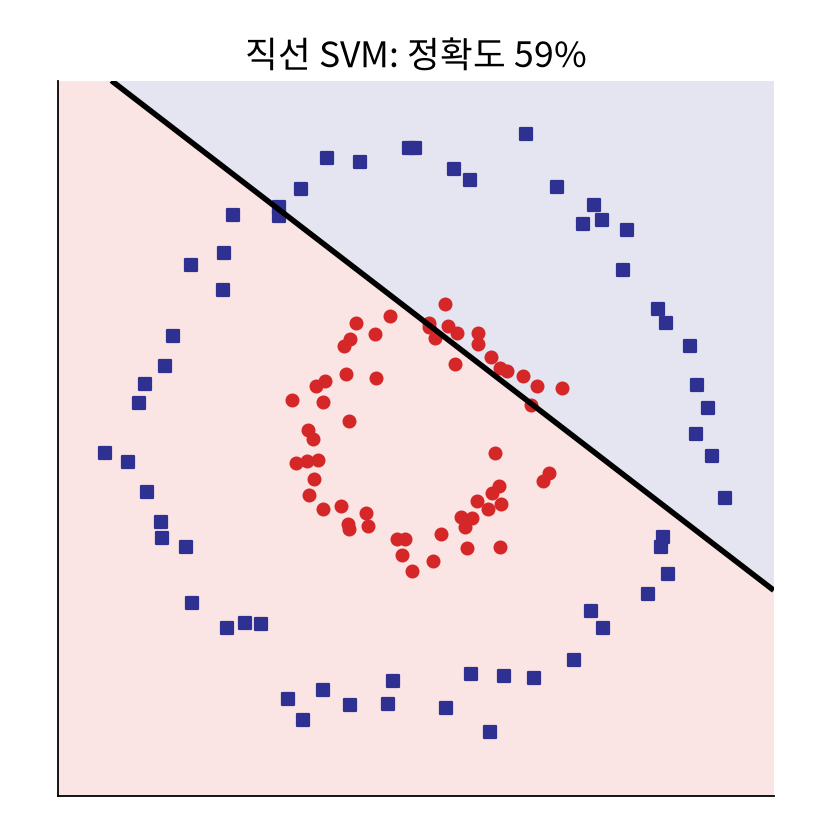
\includegraphics[width=0.95\linewidth]{kn_q.png}\end{column}
\begin{column}{0.52\textwidth}
{\large 빨강이 가운데, 파랑이 바깥}\\[0.8em]
{\Large \kq{직선 말고 휘어진 경계는\\ 어떻게 만들까?}}
\end{column}
\end{columns}
\vfill
\note{빨간 점이 가운데 모여 있고 파란 점이 바깥을 둘러싼 데이터입니다. 지난 시간의 선형 SVM으로 학습하면 어떤 직선을 그어도 반쯤밖에 못 맞혀서, 정확도가 59퍼센트입니다. 경계가 원이어야 하는데 직선만 그을 수 있기 때문입니다. 오늘은 SVM으로 휘어진 경계를 만드는 방법, 특징 늘리기와 커널을 배웁니다.}
\end{frame}

\section{특징 늘리기}
% --- 1차원 → 2차원
\begin{frame}{가장 쉬운 예: 1차원 점에 $x^2$ 을 붙이면}
\vfill
\centering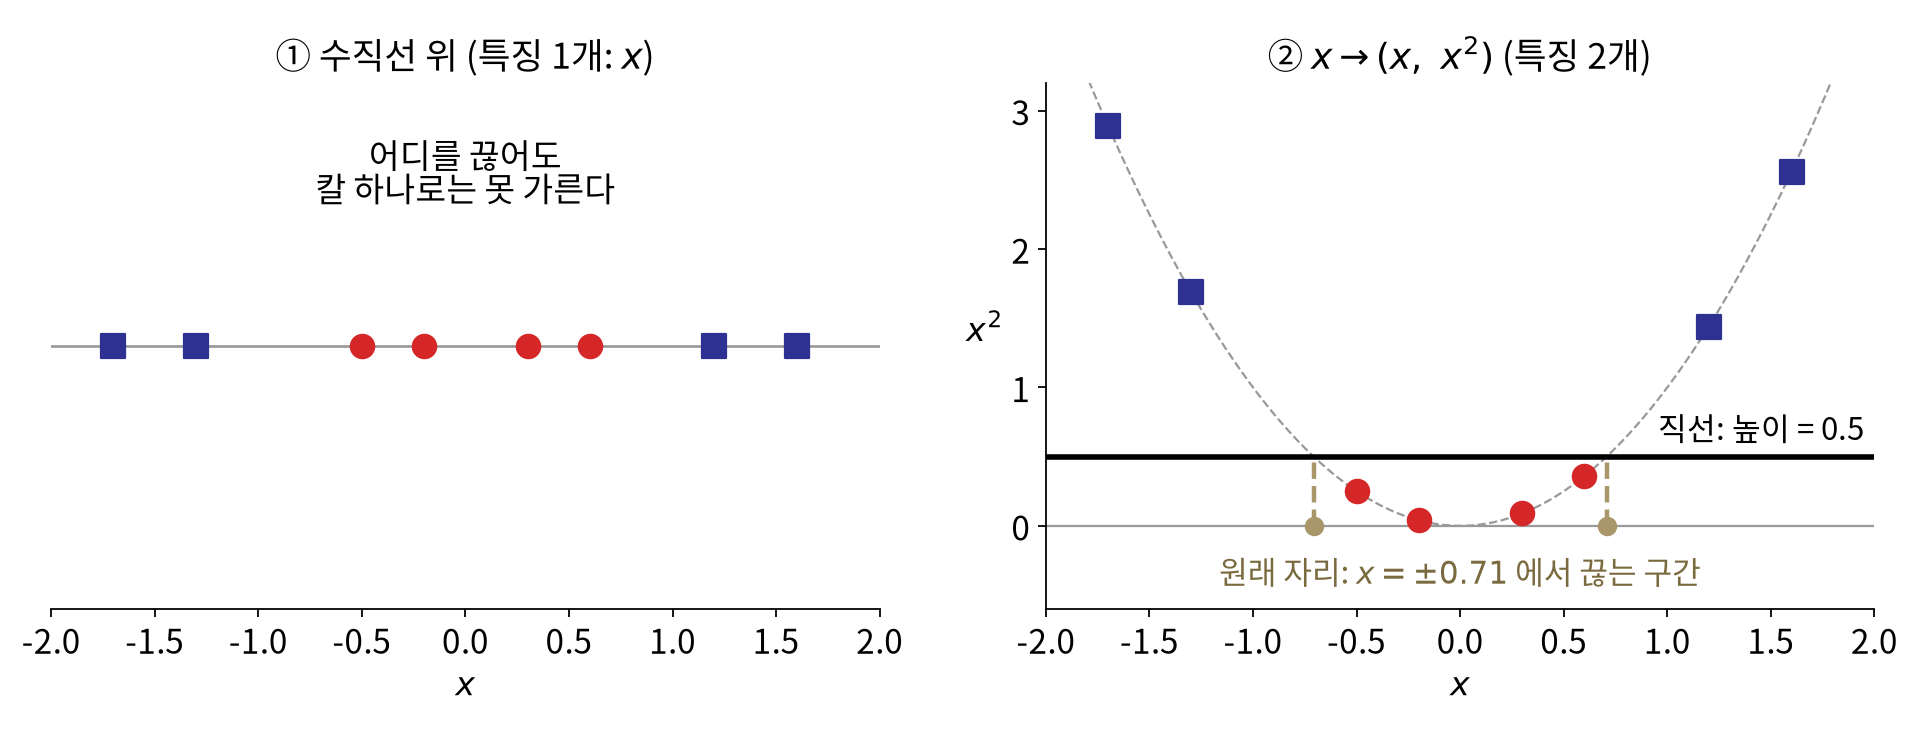
\includegraphics[width=0.9\linewidth]{kn_lift1d.png}\par\vskip0.3em
{\large 특징을 늘리면: 올린 곳에서는 \kb{직선 하나}, 원래 자리에서는 \kq{휘어진 경계} (여기선 구간)}\\[0.2em]
{\normalsize 점마다 $x^2$ 을 계산해서 붙였다 $\to$ \kb{2차원 점}}
\vfill
\note{특징 늘리기를 가장 쉬운 1차원에서 봅시다. 왼쪽은 수직선 위의 점입니다. 빨강이 가운데, 파랑이 양쪽에 있어서, 경계점 하나, 칼질 한 번으로는 어디를 끊어도 가를 수 없습니다. 이제 점마다 숫자를 하나 더 붙입니다. x 제곱입니다. 그러면 점 x가 x, x 제곱, 두 숫자가 되어 오른쪽처럼 평면 위, 포물선 위에 올라갑니다. 가운데 빨강은 낮고 양쪽 파랑은 높습니다. 이제 높이 0.5인 직선 하나로 갈라집니다. 이 직선을 원래 수직선으로 내려 보면, x 제곱이 0.5인 곳, x가 플러스 마이너스 0.71인 두 곳에서 끊는 구간이 됩니다. 특징 수는 점 하나를 숫자 몇 개로 나타내느냐입니다. 1개였던 특징을 2개로 늘리니, 늘린 공간에서는 직선이고 원래 자리에서는 휘어진 경계가 됐습니다. 다음 쪽은 2차원 점에 숫자를 하나 더 붙여 3차원으로 올리는 같은 이야기입니다.}
\end{frame}

% --- 원 모양 데이터
\begin{frame}{특징 늘리기: 직선으로 못 가르면 높이를 준다}
\markpage{lift}
\vfill
\centering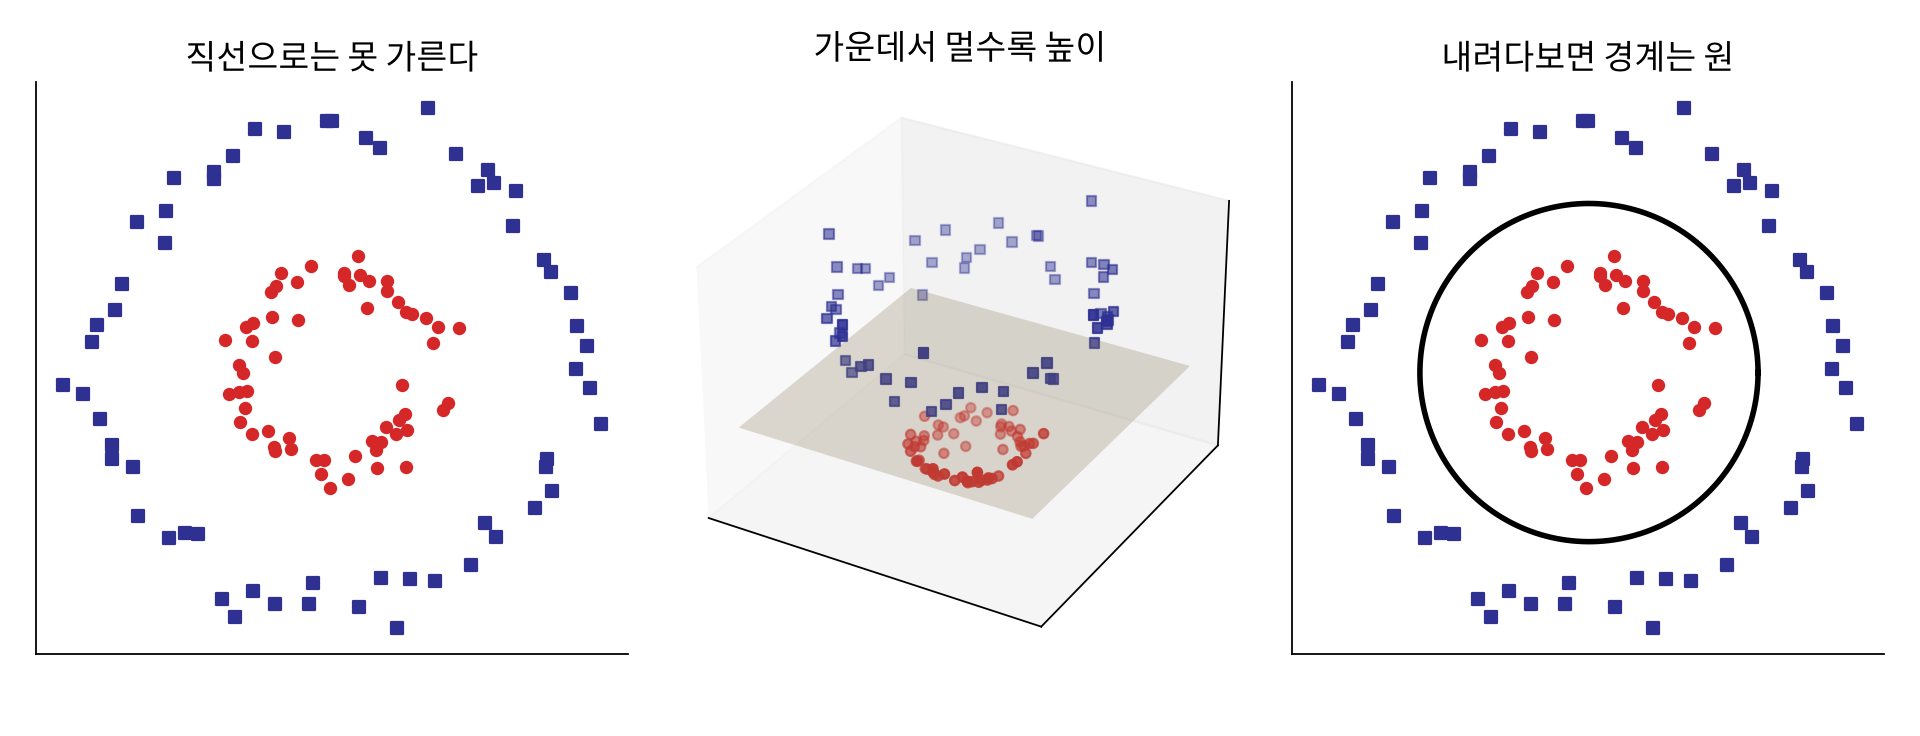
\includegraphics[width=0.86\linewidth]{sv_lift.png}\par\vskip0.2em
{\large $(x_1,\ x_2) \;\to\; (x_1,\ x_2,\ \textcolor{ksablue}{x_1^2 + x_2^2})$}\\[0.2em]{\normalsize 점마다 높이 $x_1^2 + x_2^2$ 를 계산해서 붙였다 $\to$ \kb{3차원 점}}
\vfill
\note{이번에는 빨간 점이 가운데, 파란 점이 바깥을 둘러싼 데이터입니다. 어떤 직선을 그어도 가를 수 없습니다. 그런데 각 점에 높이를 하나 더 줘 봅시다. 가운데서 떨어진 거리의 제곱, x1 제곱 더하기 x2 제곱입니다. 그러면 가운데 빨간 점은 낮게, 바깥 파란 점은 높게 떠서, 가운데 그림처럼 수평한 평면 하나로 깔끔하게 갈라집니다. 이 평면을 원래 평면에서 내려다보면 오른쪽처럼 원이 됩니다. 높은 차원에서 직선으로 가르면, 원래 차원에서는 휘어진 경계가 됩니다. 선형회귀에 x 제곱 특징을 넣은 것과 같은 아이디어입니다. 주의할 점은, 여기서는 세 번째 숫자를 우리가 점마다 실제로 계산해서 붙였다는 것입니다. 정말로 3차원 점을 만든 것이고, 이것은 커널이 아니라 특징을 직접 만든 것입니다. 뒤에서 볼 커널은 이런 숫자를 하나도 만들지 않습니다. 그런데도 결과로 나오는 경계가, 이렇게 숫자를 만들어 올린 뒤 평면으로 가른 것과 같은 모양이 됩니다. 그래서 커널을 높은 차원으로 올린 것처럼 설명하는 것입니다.}
\end{frame}

\section{커널}
% --- α 학습
\begin{frame}{$\mathbf{w}$ 는 학습 점을 더한 것: 지난 시간 학습을 $\alpha$ 로 다시 쓴다}
\vfill
\centering
\renewcommand{\arraystretch}{1.45}
{\normalsize\begin{tabular}{l|l|l}
 & 지난 시간: $\mathbf{w}$ 를 들고 & 오늘: $\alpha$ 를 들고 (\kb{점마다 하나})\\ \hline
처음 & $\mathbf{w} = 0$ & $\alpha_k = 0$ (모든 점)\\
1. 값 & $y_k D(\mathbf{x}_k) = y_k(\mathbf{w}\cdot\mathbf{x}_k + b)$ & $y_k\big(\sum_l \alpha_l y_l\, \mathbf{x}_l\cdot\mathbf{x}_k + b\big)$\\
2. 밀기 (가장 작은 점 $k$) & $\mathbf{w}' = \mathbf{w} + \eta\, y_k \mathbf{x}_k$ & $\alpha_k \leftarrow \alpha_k + \eta$\\
 & $b' = b + \eta\, y_k$ & $b' = b + \eta\, y_k$ (같다)\\
3. 길이 1 로 & $\mathbf{w} \leftarrow \mathbf{w}'/\lVert\mathbf{w}'\rVert$ & \kb{모든} $\alpha$ 를 $\lVert\mathbf{w}'\rVert$ 로 나눈다\\ \hline
끝 & $\mathbf{w}$ & $\mathbf{w} = \sum_k \alpha_k y_k \mathbf{x}_k$
\end{tabular}}\\[0.6em]
{\large $\alpha_k$ = 점 $k$ 가 지금까지 \kb{민 양} (늘 0 이상) \quad 안 미는 점은 나눠지기만 해서 \kq{0 으로}}\\[0.3em]
{\small $\lVert\mathbf{w}'\rVert^2 = \sum_k \sum_l \alpha_k \alpha_l\, y_k y_l\, \mathbf{x}_k\cdot\mathbf{x}_l$ \;$\to$\; 1 · 3 모두 \kb{점곱만} 쓴다}
\vfill
\note{커널로 가기 전에, 지난 시간에 학습한 w가 사실 무엇인지 봅시다. 지난 시간의 학습 한 걸음을 w 대신 점마다 숫자 하나, 알파로 다시 써 보겠습니다. 핵심은 w가 늘 학습 점에 숫자를 곱해 더한 꼴이라는 것입니다. w는 0에서 출발합니다. 0은 모든 알파가 0인 것과 같습니다. 밀기는 w에 에타 y k x k를 더하는 것이니, 점 k의 숫자 알파 k에 에타를 더하는 것과 같습니다. 원 논문처럼 알파는 미는 양이라 늘 0 이상이고, 빨강인지 파랑인지는 라벨 y k가 따로 맡습니다. 길이를 1로 맞추는 것은 w 전체를 길이로 나누는 것이니, 모든 알파를 같은 수로 나누는 것과 같습니다. 그래서 매 걸음이 끝나도 w는 여전히 알파 k 곱하기 y k 곱하기 x k의 합입니다. 즉 w를 들고 다니는 대신 점마다 숫자 하나, 알파를 들고 다녀도 똑같은 학습입니다. 값을 잴 때 w 점곱 x k는 알파 l 곱하기 y l 곱하기 x l 점곱 x k의 합으로 계산하고, 길이 w 프라임은 알파끼리, 점끼리의 점곱으로 계산합니다. 그래서 알파는 점 k가 지금까지 민 양입니다. 경계 가장자리에서 계속 미는 점, 서포트 벡터는 알파가 계속 쌓이고, 한 번도 안 밀거나 처음에만 민 점은 3번에서 매번 나눠지기만 해서 0으로 줄어듭니다. 이 학습 어디에도 w가 직접 필요하지 않고, 점끼리의 점곱만 쓴다는 점이 중요합니다. 원 논문은 같은 알파를 라그랑주 승수로 유도하고, 식 16에서 w 별이 알파 k y k x k의 합이라는 것을 보입니다. sklearn은 SMO라는 방법으로 알파를 두 개씩 고쳐 가며 풉니다. 풀이법은 다르지만 같은 답이 나옵니다.}
\end{frame}

% --- α 가 쌓이는 모습
\begin{frame}{$\alpha$ 가 쌓이는 모습: 서포트 벡터 3개만 남는다}
\vfill
\centering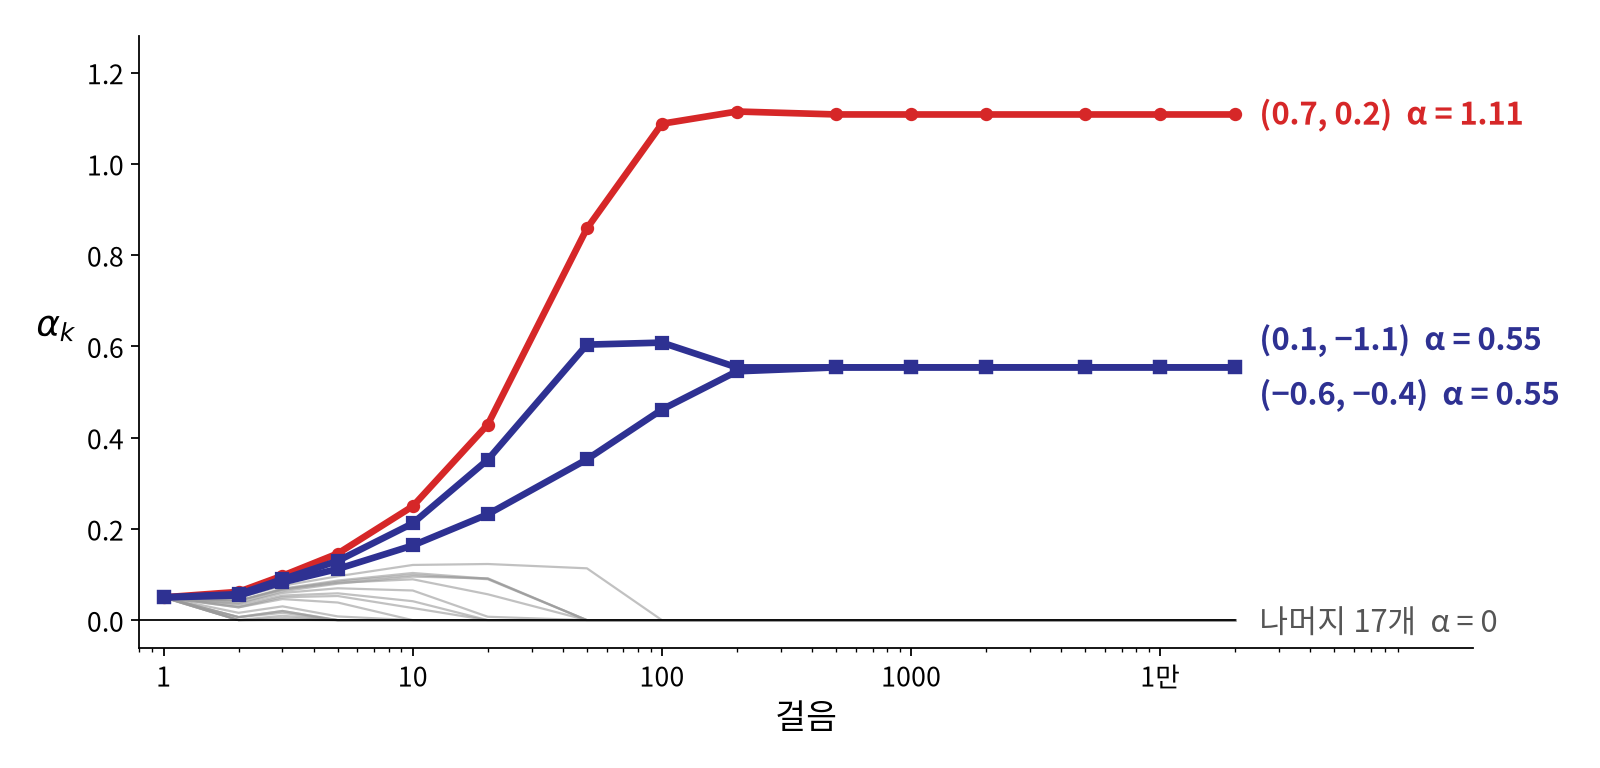
\includegraphics[width=0.72\linewidth]{kn_alpha.png}\par\vskip0.2em
{\large 2만 걸음: $0.74$ · $0.37$ · $0.37$, 나머지 17개 \kb{0}}\\[0.2em]
{\normalsize $M = 0.67$ 로 나누면 (가장자리 $D(\mathbf{x}) = \pm 1$ 기준) \;$\alpha^* = $ \kb{$1.1$ · $0.55$ · $0.55$} \;= sklearn}
\vfill
\note{지난 시간 점 20개로 알파 학습을 실제로 돌려 본 것입니다. 가로축은 걸음, 로그 눈금입니다. 첫 걸음에서는 모든 점의 값이 0으로 같아서 20개가 다 함께 밀고, 알파가 모두 0.04 정도입니다. 그 뒤로는 가장 가까운 점만 밀어서, 빨간 0.7, 0.2는 10걸음에 0.14, 100걸음에 0.36, 1000걸음에 0.66으로 쌓이고, 파란 두 점도 쌓입니다. 회색 선 17개는 처음 한 번 민 뒤로 다시 밀지 않아서 나눠지기만 하고, 100걸음에 0.02, 1000걸음에 0.005, 2만 걸음에는 0이 됩니다. 2만 걸음 뒤 알파는 0.74, 0.37, 0.37입니다. 이것은 w의 길이를 1로 둔 기준의 값입니다. 지난 시간 끝에서 본 것처럼 원 논문과 sklearn은 가장 가까운 값을 1로 두는데, 그러면 w와 b를 마진 M 0.67로 나누니 알파도 0.67로 나눕니다. 그러면 1.1, 0.55, 0.55, sklearn이 낸 알파와 같습니다. 여기부터는 이 값을 알파 별이라고 부르고 씁니다. 그래서 w는 서포트 벡터 세 개에 알파를 곱해 더한 것입니다. 나머지 17개 점은 w에 들어가지 않습니다.}
\end{frame}

% --- 서포트 벡터 화살표
\begin{frame}{$\mathbf{w}$ = 서포트 벡터끼리의 화살표}
\vfill
\centering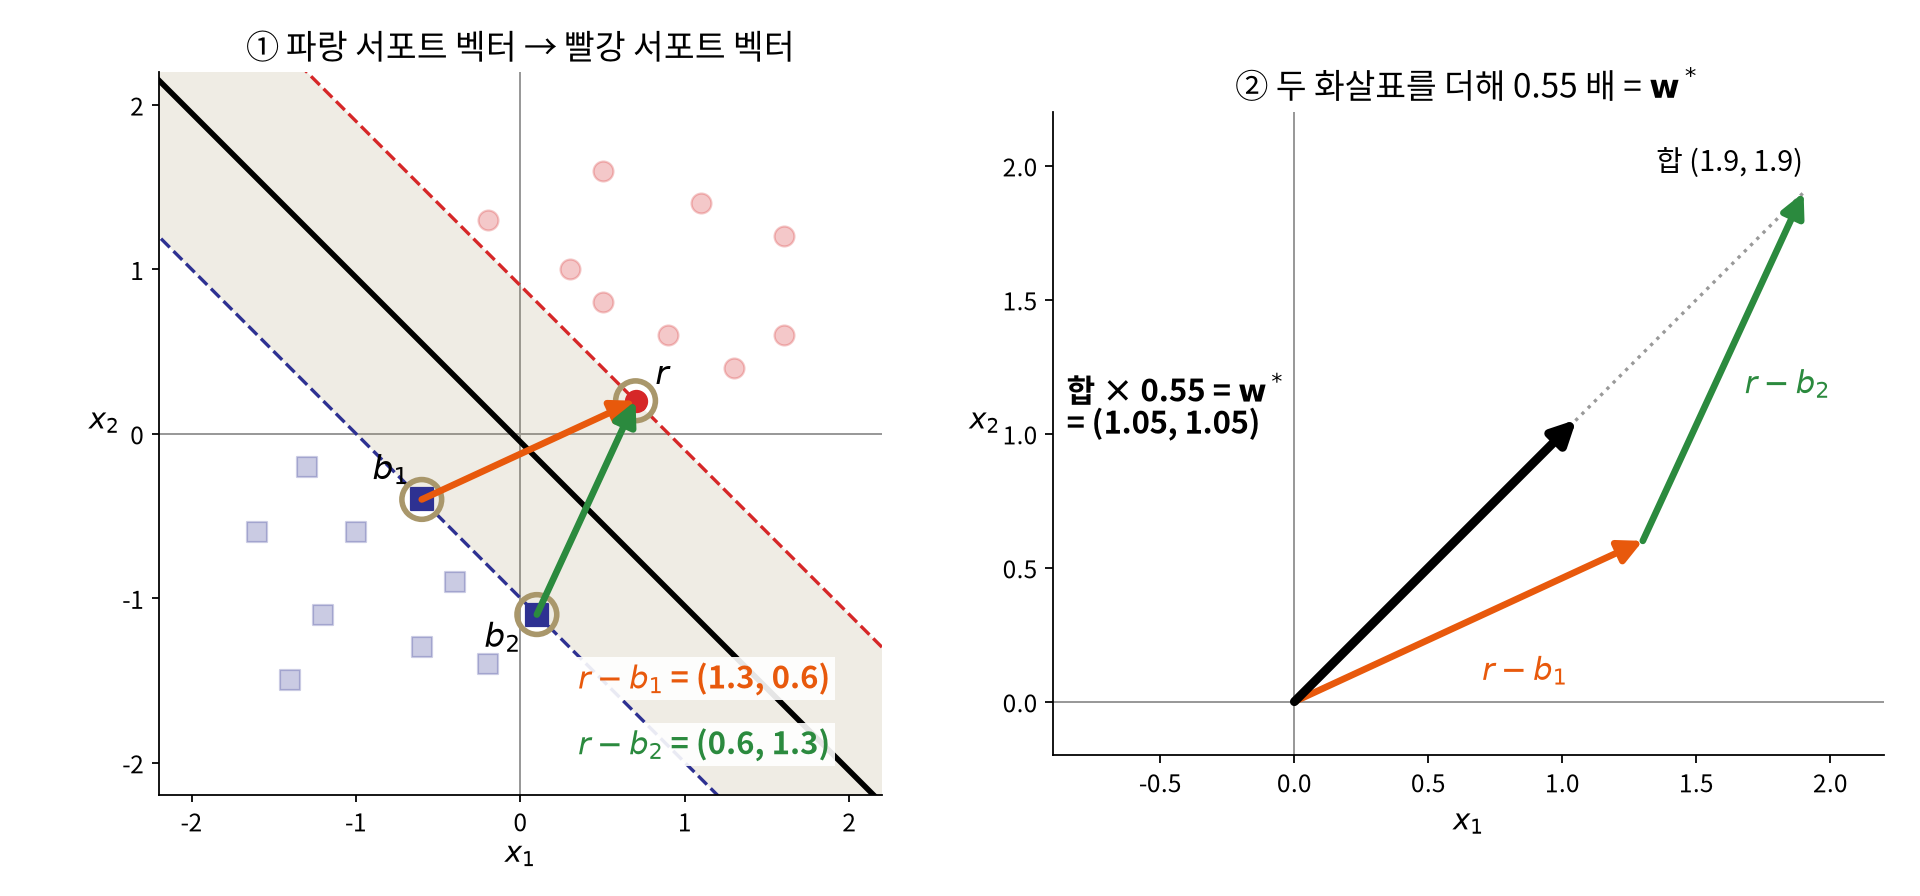
\includegraphics[width=0.78\linewidth]{kn_svarrow.png}\par\vskip0.1em
{\large $\mathbf{w}^* = \sum_k \alpha_k y_k \mathbf{x}_k = 1.1\, r - 0.55\, b_1 - 0.55\, b_2 = 0.55\,\big[(r - b_1) + (r - b_2)\big] = (1.05,\ 1.05)$}\\[0.2em]
{\normalsize 빨강 무게 $1.1$ = 파랑 무게 $0.55 + 0.55$ \;$\to$\; \kb{파랑 $\to$ 빨강 화살표}로 묶인다}
\vfill
\note{학습이 끝난 w를 서포트 벡터 세 개로 다시 봅시다. 빨간 서포트 벡터를 r, 파란 두 개를 b1, b2라고 부르겠습니다. w 별은 알파 k 곱하기 y k 곱하기 x k의 합이니, 빨강은 y가 플러스 1, 파랑은 마이너스 1이라 1.1 곱하기 r 빼기 0.55 곱하기 b1 빼기 0.55 곱하기 b2입니다. 빨강 쪽 무게 1.1이 파랑 쪽 무게 0.55 더하기 0.55와 같기 때문에, 이 식은 0.55 곱하기, r 빼기 b1 더하기 r 빼기 b2로 묶을 수 있습니다. r 빼기 b1은 왼쪽 그림의 주황 화살표, 파란 b1에서 빨간 r로 가는 화살표이고 1.3, 0.6입니다. r 빼기 b2는 초록 화살표, b2에서 r로 가는 화살표이고 0.6, 1.3입니다. 오른쪽 그림처럼 두 화살표를 꼬리에 이어 더하면 1.9, 1.9이고, 0.55를 곱하면 1.05, 1.05, 바로 w 별입니다. 즉 w는 파랑 서포트 벡터에서 빨강 서포트 벡터로 가는 화살표를 더한 방향입니다. 파랑에서 빨강 쪽을 가리키니 경계의 방향이 되는 것이 자연스럽습니다. 확인해 보면 파랑 길 가장자리는 b1과 b2를 지나고 방향이 b2 빼기 b1, 0.7, 마이너스 0.7인데, w와 점곱하면 0이라 w는 길 가장자리와 수직입니다. 또 r 빼기 b1을 w 방향으로 재면 1.9 곱하기 0.71, 1.34로 길 폭과 같습니다. 멀리 있는 17개 점은 지우거나 옮겨도 경계가 그대로이니, 답의 식에 들어갈 이유가 없고 알파가 0입니다. 그래서 w는 서포트 벡터끼리의 빼기와 더하기로 써집니다.}
\end{frame}

% --- 역학 비유
\begin{frame}{역학으로 보면: $\alpha$ = 서포트 벡터가 경계를 미는 힘}
\vfill
\centering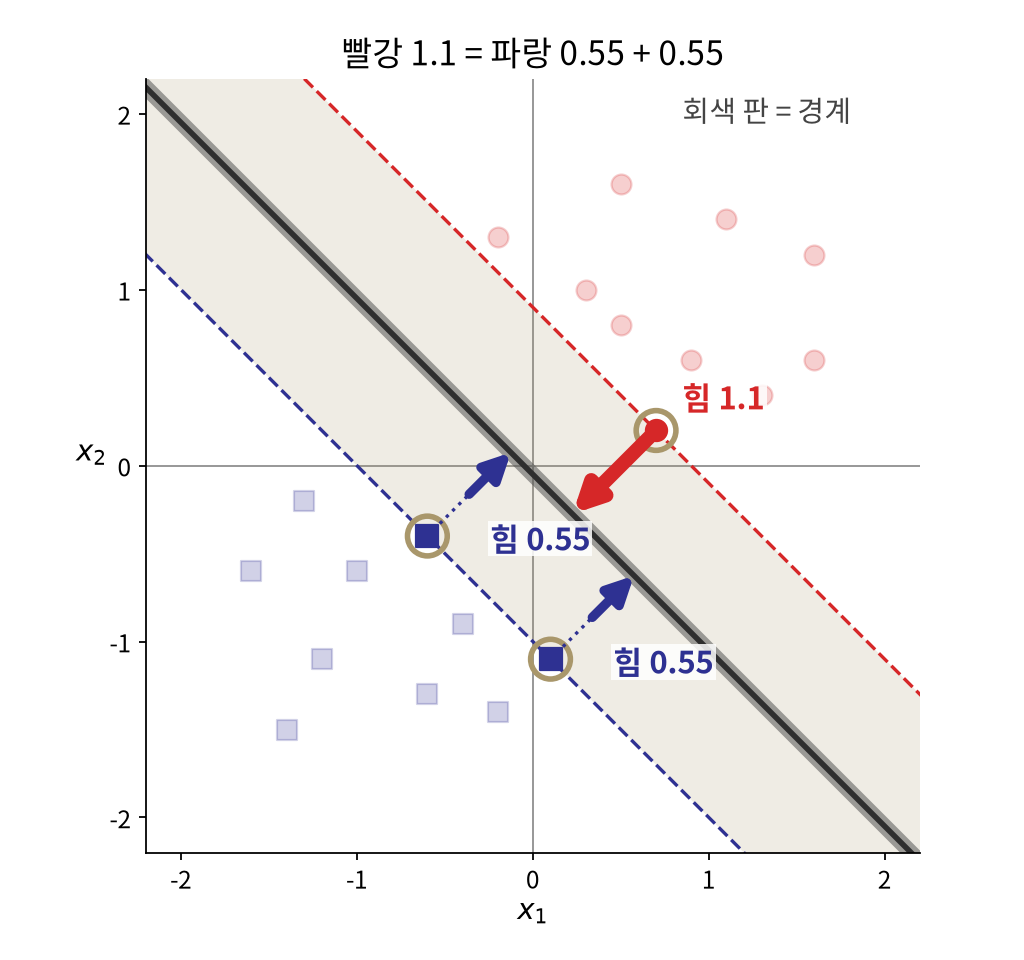
\includegraphics[height=0.62\textheight]{kn_force.png}\par\vskip0.2em
{\large 양쪽 힘이 같다 \ $1.1 = 0.55 + 0.55$, \;$\sum_k \alpha_k y_k = 0$ \;$\to$\; 경계가 \kb{멈춘다}}\\[0.2em]
{\normalsize 서포트 벡터 = 길을 \kq{받치는} 점 (support), \ 나머지 17개는 힘 0}
\vfill
\note{알파를 힘으로 보는 역학 비유가 있습니다. 경계를 딱딱한 판이라고 생각합시다. 서포트 벡터가 이 판을 밉니다. 빨간 서포트 벡터는 파랑 쪽으로, 파란 서포트 벡터 둘은 빨강 쪽으로 밉니다. 미는 힘의 크기가 알파이고, 미는 방향이 라벨 y입니다. 빨강은 1.1, 파랑은 각각 0.55입니다. 판이 어느 쪽으로도 밀려 가지 않으려면 양쪽 힘이 같아야 합니다. 1.1은 0.55 더하기 0.55와 같고, 알파 k 곱하기 y k를 다 더하면 0입니다. 원 논문에서는 b까지 최적으로 고르면 이 합이 0이 된다는 식으로 나옵니다. 판이 돌지도 않습니다. 경계를 따라 잰 위치에 힘을 곱한 돌림힘을 더해 보면, 빨강은 위치 마이너스 0.35에 힘 1.1, 파랑은 위치 0.14와 마이너스 0.85에 힘 0.55씩이라, 0.39 더하기 0.08 빼기 0.47로 0입니다. 그래서 이 자리에서 판이 멈춥니다. 서포트 벡터라는 이름도 여기서 옵니다. 길의 가장자리를 받쳐서, support해서, 길이 더 넓어지지 못하게 막는 점들입니다. 나머지 17개 점은 판을 밀지 않습니다. 힘이 0, 알파가 0입니다. 원 논문 식 15가 이것입니다. 가장자리에 닿지 않은 점은 알파가 0입니다. 지워도 판이 그대로입니다. 이 비유는 Burges가 1998년에 쓴 SVM 튜토리얼에 나옵니다. 지난 시간 학습에서 가장 가까운 점이 민다고 했던 것이 바로 이 힘이 쌓이는 과정입니다.}
\end{frame}

% --- 선형 SVM 을 점곱으로
\begin{frame}{$\mathbf{w} = \sum_k \alpha_k y_k \mathbf{x}_k$ 를 분류기에 넣으면: 새 점과 서포트 벡터의 점곱}
\vfill
\centering
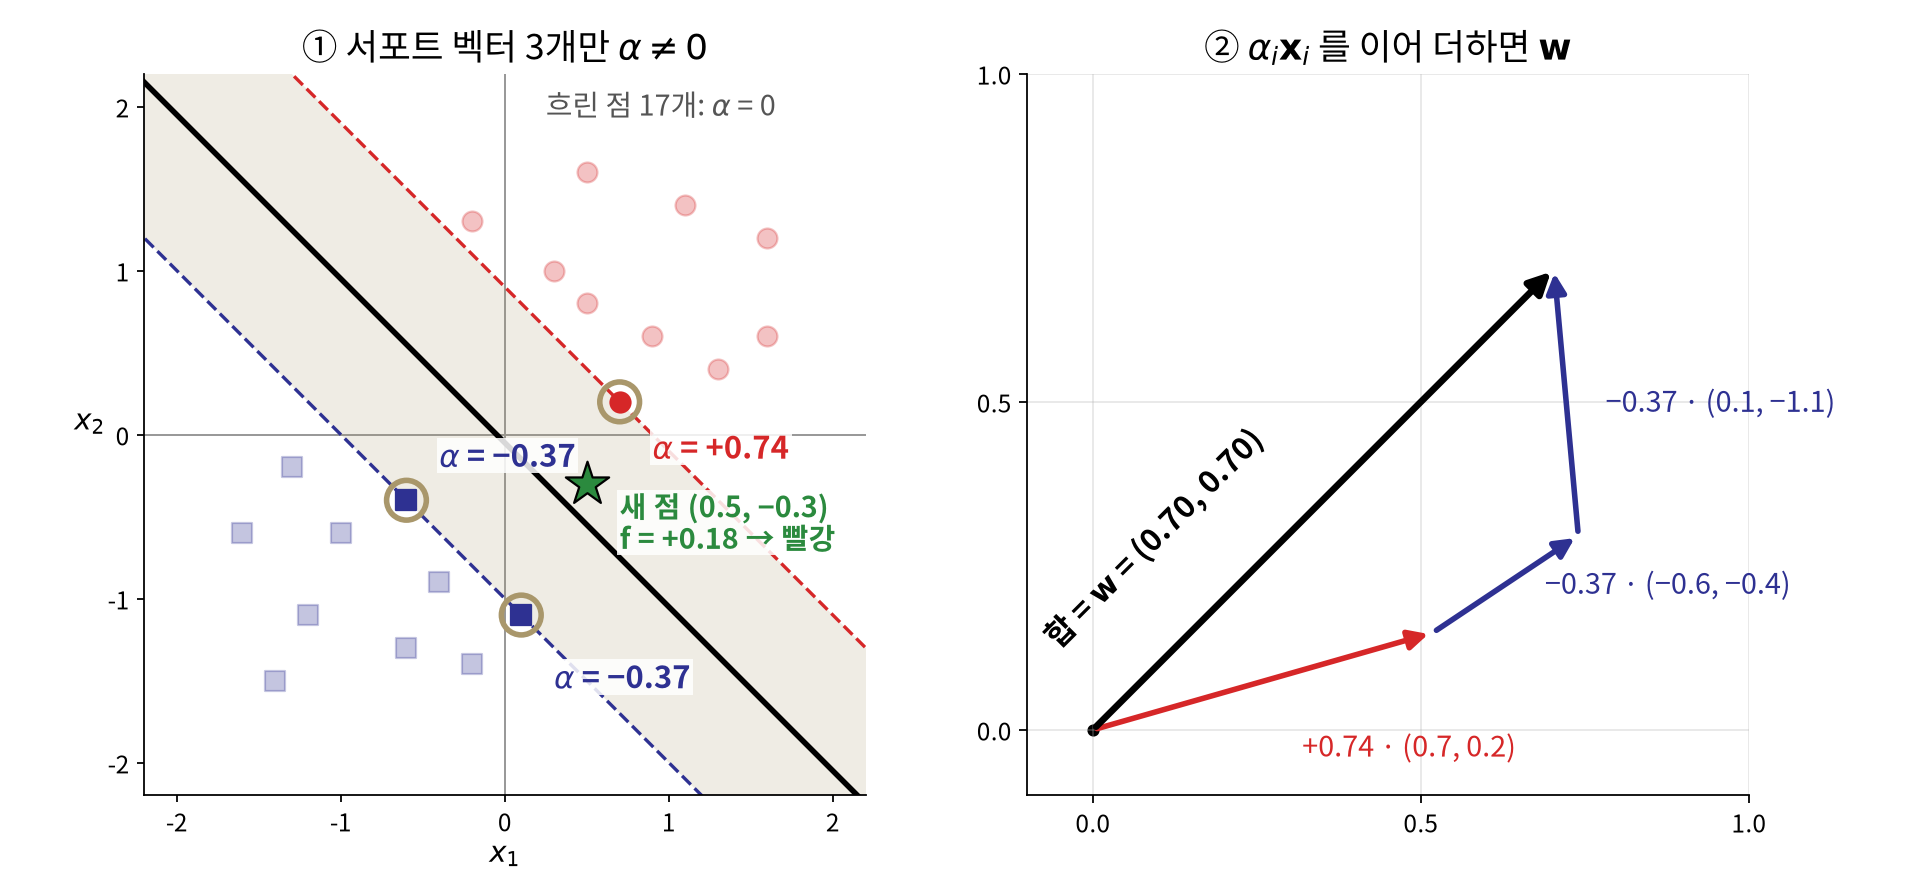
\includegraphics[width=0.62\linewidth]{kn_dual.png}\par\vskip0.1em
{\large $D(\mathbf{x}) = \mathbf{w}\cdot\mathbf{x} + b = \big(\sum_{k} \alpha_k y_k \mathbf{x}_k\big)\cdot\mathbf{x} + b = b + \sum_{k} \alpha_k y_k\, \mathbf{x}\cdot\mathbf{x}_k$}\\[0.1em]
{\normalsize 예 $\star$: \; $\mathbf{w}^*\cdot\mathbf{x} = 0.21$ (한 번에) $= 0.32 + 0.10 - 0.21$ (나눠서) $\to$ $D(\mathbf{x}) = +0.26$ \kq{빨강}}\\[0.1em]
{\small $\mathbf{x}$ = 분류할 새 점, \; $\mathbf{x}_k$ = 서포트 벡터 ($\alpha_k \neq 0$ 인 점만 남는다)}
\vfill
\note{방금 본 대로 w는 서포트 벡터에 알파와 y를 곱해 더한 것입니다. 이것을 분류기 D x, w 점곱 x 더하기 b에 넣어 봅시다. 왼쪽 그림에서 진한 점 3개가 서포트 벡터이고, 옆의 숫자가 그 점의 알파입니다. 빨간 서포트 벡터 0.7, 0.2는 알파가 1.1, 파란 둘은 0.55입니다. 흐리게 그린 나머지 17개는 알파가 0입니다. 경계를 정하는 데 쓰이지 않는 점들입니다. 오른쪽 그림은 알파 곱하기 y 곱하기 점을 화살표로 이어 붙인 것입니다. 빨강은 y가 플러스 1이라 그대로, 파랑은 마이너스 1이라 반대 방향입니다. 1.1 곱하기 0.7, 0.2에서 시작해 마이너스 0.55 곱하기 마이너스 0.6, 마이너스 0.4를 잇고, 마이너스 0.55 곱하기 0.1, 마이너스 1.1을 이으면, 끝점이 1.05, 1.05, 바로 w 별입니다. 그래서 w 점곱 x 더하기 b는 b 더하기 알파 k 곱하기 y k 곱하기 x 점곱 x k의 합으로 쓸 수 있습니다. 여기서 x는 분류하려는 새 점 하나, x k는 서포트 벡터 하나이고, 점곱은 숫자 하나입니다. 원 논문 식 18이 이 꼴입니다. 초록 별, 0.5, 마이너스 0.3을 분류해 봅시다. 빨간 서포트 벡터 0.7, 0.2와의 점곱은 0.35 빼기 0.06, 0.29이고 알파 1.1을 곱하면 0.32입니다. 파란 마이너스 0.6, 마이너스 0.4와의 점곱은 마이너스 0.18, 알파 0.55와 y 마이너스 1을 곱하면 0.10입니다. 파란 0.1, 마이너스 1.1과의 점곱은 0.38, 알파와 y를 곱하면 마이너스 0.21입니다. 더하면 0.21이고 b 별 0.05를 더하면 D는 0.26, 0보다 크니 빨강입니다. w 별 1.05, 1.05로 한 번에 계산해도 1.05 곱하기 0.5 더하기 1.05 곱하기 마이너스 0.3, 0.21로 같습니다. 이 기준에서 값은 거리가 아니라 가장 가까운 점을 1로 둔 눈금이라, 거리는 0.26 곱하기 마진 0.67, 0.18입니다. 왜 w 점곱 x가 이렇게 나뉠까요? 점곱은 더하기를 나눠서 할 수 있으니, 합 전체와 x의 점곱은 서포트 벡터마다 따로 계산해서 더한 것과 같습니다. 같은 값을 w로 한 번에 계산하느냐, 서포트 벡터마다 나눠 계산하느냐의 차이일 뿐입니다. 나눠 쓴 꼴에는 w가 없고 새 점과 서포트 벡터의 점곱만 남습니다. 이 점곱 자리를 바꾸는 것이 다음 쪽 커널입니다.}
\end{frame}

% --- 커널 트릭
\begin{frame}{커널: 점곱 자리에 $K$ 를 넣는다}
\markpage{kernel}
\vfill
\centering
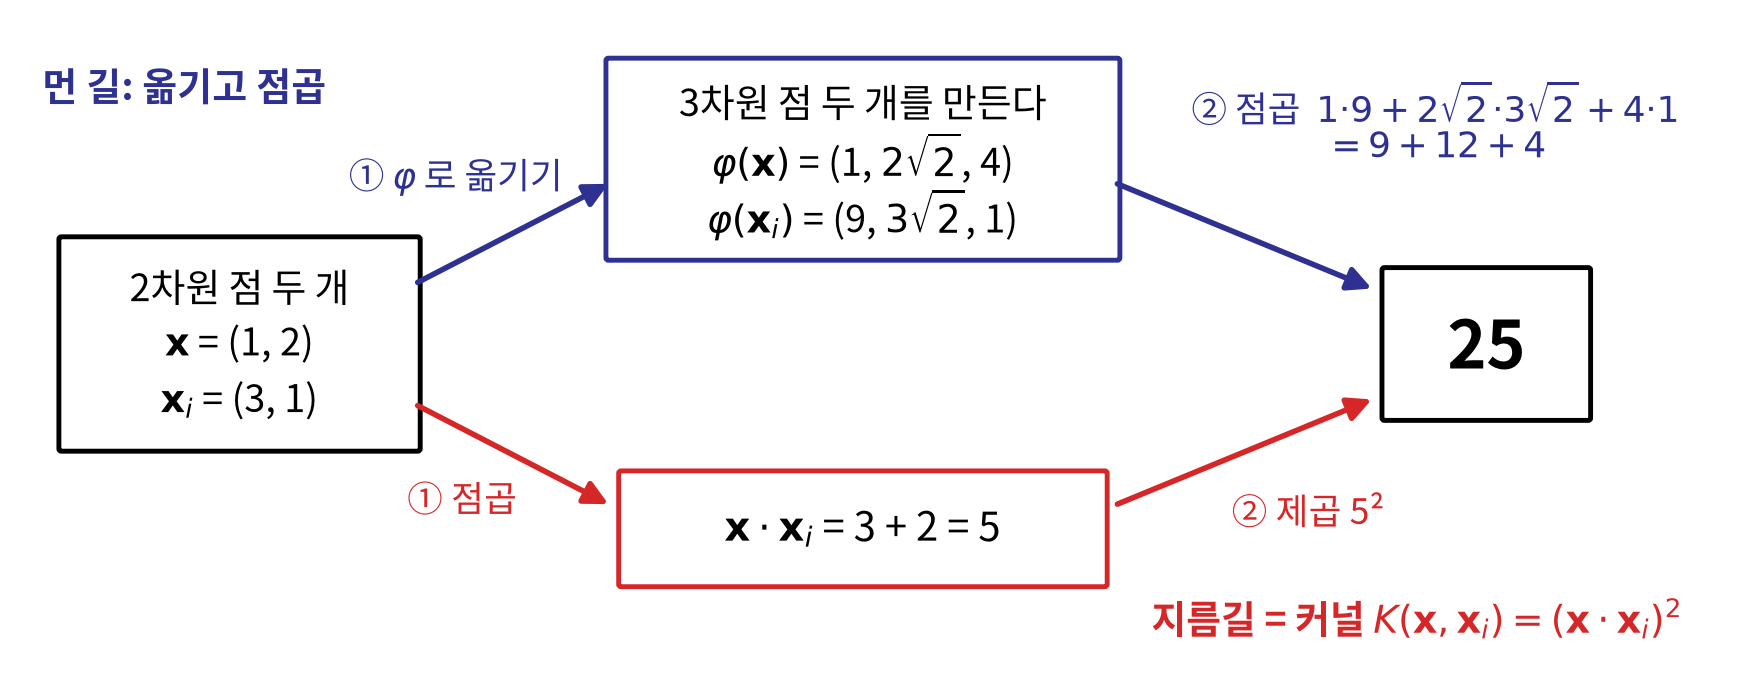
\includegraphics[width=0.8\linewidth]{kn_ktrick.png}\par\vskip0.2em
{\large $D(\mathbf{x}) = b + \sum_{k} \alpha_k y_k\, \mathbf{x}\cdot\mathbf{x}_k$ \;$\to$\; $D(\mathbf{x}) = b + \sum_{k} \alpha_k y_k\, \textcolor{ksablue}{\boldsymbol{K}(\mathbf{x}, \mathbf{x}_k)}$}\\[0.2em]
{\normalsize $\varphi(\mathbf{x}) = (x_1^2,\ \sqrt2\,x_1x_2,\ x_2^2)$ 로 옮긴 뒤의 점곱을, 옮기지 않고 \kb{지름길}로 계산}
\vfill
\note{앞 쪽 식에서 점곱 자리에 다른 함수 K를 넣은 것이 커널 SVM입니다. 이 K를 커널이라고 부릅니다. 커널은 점들을 높은 차원으로 옮긴 뒤의 점곱을, 실제로 옮기지 않고 원래 점으로 바로 계산하는 함수입니다. 순서를 바꿔도 값이 같고, 두 점이 가까울수록 큰 값을 내서 유사도처럼 읽을 수 있습니다. 예를 들어 2차원 점을 x1 제곱, 루트2 x1 x2, x2 제곱인 3차원으로 옮기면, 옮긴 뒤의 점곱은 원래 점곱의 제곱과 정확히 같습니다. 이름은 앞 쪽 식에 맞춰 x는 새 점, x k는 서포트 벡터 같은 학습 점입니다. 그림의 위쪽 파란 길은 먼 길입니다. x 1, 2와 x k 3, 1을 각각 3차원 점 1, 2루트2, 4와 9, 3루트2, 1로 실제로 옮긴 뒤 점곱하면 1 곱하기 9, 2루트2 곱하기 3루트2, 4 곱하기 1입니다. 가운데는 2 곱하기 3이 6, 루트2 곱하기 루트2가 2라서 12입니다. 그래서 9 더하기 12 더하기 4, 25입니다. 아래쪽 빨간 길은 지름길입니다. 원래 점끼리 점곱하면 3 더하기 2, 5이고, 이것을 제곱하면 25입니다. 같은 값이 나오는데, 아래 길은 3차원 점을 만들지 않습니다. 이 지름길 함수, 점곱의 제곱이 커널 K입니다. 앞 쪽 식의 x 점곱 x k 자리에 K를 넣으면 커널 SVM입니다. 원 논문 식 4와 18이 바로 이 꼴입니다. 특징이 수천 개로 늘어나도 원래 점곱 하나로 계산하니, 특징을 직접 만드는 것보다 훨씬 가볍습니다. 이것이 커널 트릭입니다.}
\end{frame}

% --- 커널 SVM 학습
\begin{frame}{커널 SVM 학습: 학습에서도 점곱 자리에 $K$}
\vfill
\centering
\renewcommand{\arraystretch}{1.35}
{\large\begin{tabular}{rl}
처음 & $\alpha_k = 0$, \; $b = 0$\\
1. 값 & $y_k\big(\sum_l \alpha_l y_l\, \textcolor{ksablue}{K(\mathbf{x}_l, \mathbf{x}_k)} + b\big)$\\
2. 밀기 & 가장 작은 점 $k$: \; $\alpha_k \leftarrow \alpha_k + \eta$, \; $b \leftarrow b + \eta\, y_k$\\
3. 길이 1 로 & 모든 $\alpha$ 를 $\sqrt{\sum_k\sum_l \alpha_k\alpha_l\, y_k y_l\, \textcolor{ksablue}{K(\mathbf{x}_k, \mathbf{x}_l)}}$ 로 나눈다
\end{tabular}}\\[0.4em]
{\large 학습 내내 계산하는 건 \kq{학습 점 두 개를 넣은 $K$ 값}뿐}
\vfill
\note{앞에서 알파 학습은 점끼리의 점곱만 쓴다고 했습니다. 그러면 학습에서도 점곱 자리에 K를 넣으면 됩니다. 처음엔 알파와 b가 모두 0입니다. 첫째, 점마다 값을 잴 때 w 대신 알파 l 곱하기 y l 곱하기 K x l, x k의 합에 b를 더하고 y k를 곱합니다. 둘째, 값이 가장 작은 점이 밀어서 그 점의 알파에 에타를, b에 에타 y k를 더합니다. 셋째, 길이를 1로 맞출 때 w의 길이를 알파끼리와 K로 계산해서 모든 알파를 나눕니다. 이 과정 어디에서도 파이로 옮긴 점이나 w를 만들지 않습니다. 그래서 파이가 무한 개인 RBF도 똑같이 학습할 수 있습니다. 원 논문 식 17도 같습니다. w를 지우고 나면 알파와 b, 그리고 학습 점 두 개를 넣은 K만 남습니다. 참고로 이 학습을 직접 짜서 원 데이터 120개에 다항 커널로 2만 걸음 돌려 sklearn과 비교해 봤습니다. 마진은 둘 다 0.20, 알파가 0이 아닌 서포트 벡터도 둘 다 7개입니다. 무작위 새 점 5천 개를 두 모델로 분류하면 99.98퍼센트가 같은 답을 냅니다. sklearn은 이 문제를 SMO라는 더 빠른 방법으로 풀지만, 하는 일은 같습니다.}
\end{frame}

% --- 자주 쓰는 커널
\begin{frame}{자주 쓰는 커널}
\vfill
\centering
\renewcommand{\arraystretch}{1.35}
{\large\begin{tabular}{l|l}
선형 & $\langle \mathbf{x}, \mathbf{x}' \rangle$\\
다항 & $(\langle \mathbf{x}, \mathbf{x}' \rangle + 1)^q$\\
RBF & $\exp\!\big(-\gamma \lVert \mathbf{x}-\mathbf{x}' \rVert^2\big)$
\end{tabular}}\\[0.5em]
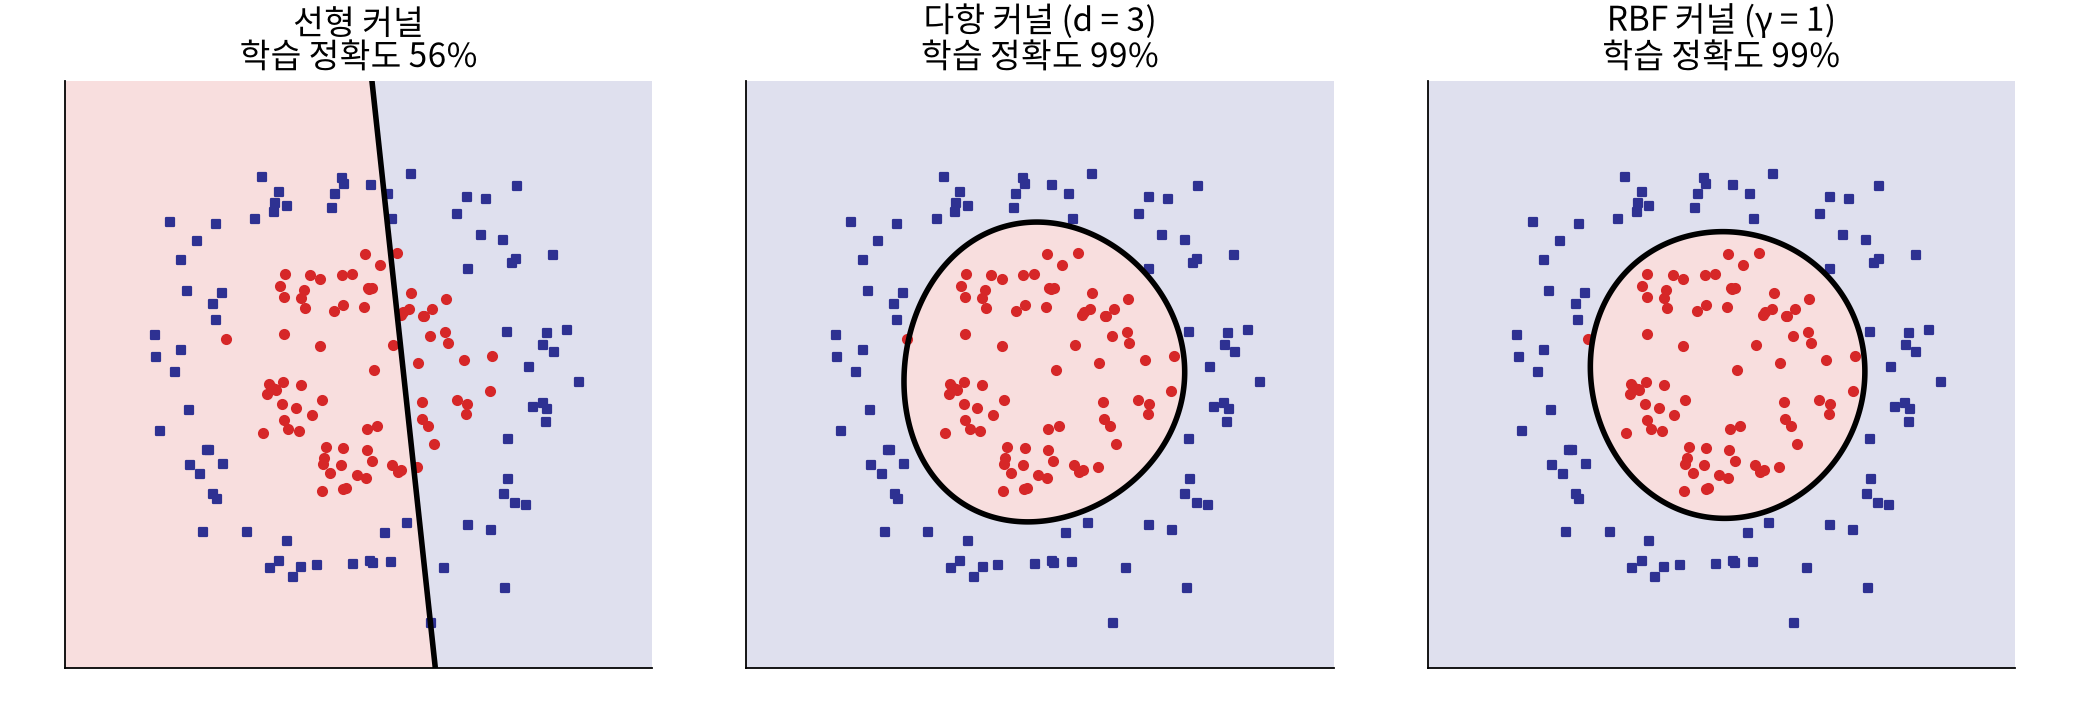
\includegraphics[width=0.8\linewidth]{sv_kernels.png}
\vfill
\note{자주 쓰는 커널은 세 가지입니다. 선형 커널은 그냥 점곱이라 앞의 서포트 벡터 분류기와 같습니다. 다항 커널은 점곱 더하기 1을 q제곱한 것으로, q차까지의 모든 곱을 특징으로 넣은 것과 같습니다. 차수를 q로 쓰는 것은 원 논문의 표기입니다. RBF 커널은 두 점 사이 거리의 제곱에 마이너스 감마를 곱해 지수를 취한 것으로, 학습 점마다 언덕을 하나씩 세워 그 높이를 특징으로 쓴 것과 같습니다. 다음 쪽 표에서 정리합니다. 아래 그림은 같은 원 모양 데이터에 세 커널을 쓴 결과입니다. 선형 커널은 직선이라 56퍼센트밖에 못 맞히고, q가 3인 다항 커널과 감마가 1인 RBF 커널은 원 모양 경계를 만들어 99퍼센트를 맞힙니다. 세 그림 모두 C는 1입니다.}
\end{frame}

% --- 세 커널 한눈에
\begin{frame}{선형 · 다항 · RBF 한눈에: 특징이 몇 개인가}
\markpage{kernels3}
\vfill
\centering
\renewcommand{\arraystretch}{1.55}
{\normalsize\begin{tabular}{c|c|c|c}
 & \textbf{선형} & \textbf{다항} ($q = 2$) & \textbf{RBF}\\ \hline
$K(\mathbf{x}, \mathbf{x}')$ & $\mathbf{x}\cdot\mathbf{x}'$ & $(\mathbf{x}\cdot\mathbf{x}' + 1)^2$ & $e^{-\gamma\lVert\mathbf{x}-\mathbf{x}'\rVert^2}$\\
특징 $\varphi(\mathbf{x})$ & $x_1,\ x_2$ & $1,\ x_1,\ x_2,\ x_1^2,\ x_1x_2,\ x_2^2$ & 모든 차수 항\\
특징 수 $N$ & 2 & 6 & \kq{$\infty$}\\
특징 직접 만들기 & 된다 & 된다 & \kq{못 한다} $\to$ \kb{커널로만}\\
경계 & 직선 & 원 · 타원 · 쌍곡선 & 어떤 모양이든\\ \hline
실제 계산 & \multicolumn{3}{c}{셋 다 $D(\mathbf{x}) = b + \sum_{k} \alpha_k y_k K(\mathbf{x}, \mathbf{x}_k)$ \;(학습 점 $p$ 개 중 서포트 벡터만)}\\ \hline
\multicolumn{4}{c}{앞의 $(x_1,\ x_2,\ x_1^2 + x_2^2)$ = 다항 2차 특징 6개 중 일부를 손으로 고른 것}
\end{tabular}}\\[0.6em]
{\small 실제 상수: 다항은 $(1, \sqrt2 x_1, \sqrt2 x_2, x_1^2, \sqrt2 x_1x_2, x_2^2)$ 이어야 점곱이 $(\mathbf{x}\cdot\mathbf{x}' + 1)^2$ 과 정확히 같다}
\vfill
\note{세 커널이 헷갈리니 한 표로 정리합니다. 기준은 하나, 특징을 몇 개 쓰는가입니다. 선형 커널은 특징을 늘리지 않습니다. x1, x2 그대로, 2개이고 경계는 직선입니다. 다항 커널 2차는 점곱 더하기 1을 제곱한 것인데, 펼쳐 보면 1, x1, x2, x1 제곱, x1 x2, x2 제곱, 이렇게 6개 특징의 점곱과 정확히 같습니다. 정확히는 루트2 같은 상수가 붙습니다. 이 6개로 직선을 그으면 원래 평면에서는 원, 타원, 쌍곡선 같은 2차 곡선이 됩니다. 앞에서 원 데이터에 높이 x1 제곱 더하기 x2 제곱을 붙였던 것은 커널이 아니라, 이 6개 중 몇 개를 손으로 골라 만든 특징 3개입니다. 그래서 원만 그릴 수 있었습니다. RBF는 펼치면 0차, 1차, 2차, 3차, 모든 차수의 항이 다 들어 있어 특징이 무한 개입니다. 무한 개라 직접 만들 수는 없습니다. 그래서 맨 아래 줄이 중요합니다. 세 커널 모두 SVM이 실제로 계산하는 것은 똑같이 b 더하기 서포트 벡터마다 알파 곱하기 y 곱하기 K입니다. 특징 공간이 2차원이든 6차원이든 무한 차원이든, 계산은 학습 점 p개 중 서포트 벡터 수만큼의 K 값으로 끝납니다. 이것이 커널 트릭입니다. 특징 수와 계산하는 항의 수는 다른 것입니다. 언덕의 폭은 감마 하나로 모두 같고, 학습은 언덕마다 높이 알파를 정하는 것이며, 대부분 0이 되어 서포트 벡터의 언덕만 남습니다. 그래서 경계는 어떤 모양이든 될 수 있습니다. 감마는 언덕 폭이지 특징 수가 아닙니다.}
\end{frame}

% --- 다항 커널 전개
\begin{frame}{왜 $(\mathbf{x}\cdot\mathbf{x}' + 1)^2$ 가 특징 6개의 점곱인가}
\vfill
\centering
\renewcommand{\arraystretch}{1.4}
{\normalsize\begin{tabular}{rl}
\textbf{1.} & 점곱 풀기: \; $\mathbf{x}\cdot\mathbf{x}' = x_1x_1' + x_2x_2'$\\
\textbf{2.} & 제곱 펼치기: \; $(x_1x_1' + x_2x_2' + 1)^2$\\
 & $= 1 + 2x_1x_1' + 2x_2x_2' + x_1^2x_1'^2 + 2x_1x_2x_1'x_2' + x_2^2x_2'^2$\\
\textbf{3.} & 항마다 ($\mathbf{x}$ 쪽) $\times$ ($\mathbf{x}'$ 쪽) 로 나누기:\\
 & $1{\cdot}1 + (\sqrt2x_1)(\sqrt2x_1') + (\sqrt2x_2)(\sqrt2x_2') + (x_1^2)(x_1'^2) + (\sqrt2x_1x_2)(\sqrt2x_1'x_2') + (x_2^2)(x_2'^2)$\\
\textbf{4.} & $\mathbf{x}$ 쪽만 모으면: \; $\varphi(\mathbf{x}) = (1,\ \sqrt2x_1,\ \sqrt2x_2,\ x_1^2,\ \sqrt2x_1x_2,\ x_2^2)$ \;$\to$ \kb{6개}, \; $K = \varphi(\mathbf{x})\cdot\varphi(\mathbf{x}')$
\end{tabular}}\\[0.7em]
{\large 예: $\mathbf{x} = (1, 2)$, $\mathbf{x}' = (3, 1)$ \quad $(5 + 1)^2 = 36$ \; $=$ \; $1 + 6 + 4 + 9 + 12 + 4$}
\vfill
\note{다항 커널이 왜 특징 6개의 점곱과 같은지 직접 펼쳐 봅시다. 첫째, 점곱은 x1 x1 프라임 더하기 x2 x2 프라임입니다. 둘째, 이것에 1을 더해 제곱해서 펼치면 여섯 항이 나옵니다. 1, 2 x1 x1 프라임, 2 x2 x2 프라임, x1 제곱 x1 프라임 제곱, 2 x1 x2 x1 프라임 x2 프라임, x2 제곱 x2 프라임 제곱. 셋째, 각 항을 x에만 관한 것과 x 프라임에만 관한 것의 곱으로 나눕니다. 2 x1 x1 프라임은 루트2 x1 곱하기 루트2 x1 프라임입니다. 2는 루트2 두 개로 나눠 양쪽에 하나씩 줍니다. 넷째, x 쪽만 모으면 1, 루트2 x1, 루트2 x2, x1 제곱, 루트2 x1 x2, x2 제곱, 6개의 특징이 되고, 커널 값은 이 6개짜리 벡터 두 개의 점곱과 정확히 같습니다. 숫자로 확인하면 x가 1, 2이고 x 프라임이 3, 1일 때 점곱은 5, 5 더하기 1의 제곱은 36입니다. 6개 특징으로 계산해도 1 더하기 6 더하기 4 더하기 9 더하기 12 더하기 4, 36입니다. 커널은 이 6개를 만들지 않고 점곱 하나, 덧셈 하나, 제곱 하나로 같은 값을 냅니다.}
\end{frame}

% --- 1차원 커널 식 풀기
\begin{frame}{커널 식을 풀어 보면: 1차원, 학습 점 2개}
\vfill
\centering
{\large $D(x) = \sum_k \alpha_k y_k\, (x\,x_k + 1)^2$ \;($b = 0$)}\\[0.2em]
{\normalsize 학습 점: \; $x = 0$ 빨강 ($y = +1$) $\alpha = 1$, \quad $x = 2$ 파랑 ($y = -1$) $\alpha = 0.25$}\\[0.4em]
\renewcommand{\arraystretch}{1.5}
{\large\begin{tabular}{rl}
커널 계산 & $D(x) = 1\cdot(+1)\cdot(0\cdot x + 1)^2 \;+\; 0.25\cdot(-1)\cdot(2x + 1)^2$\\
괄호 풀기 & $= 1 \;-\; 0.25\,(1 + 4x + 4x^2)$\\
모으기 & $=$ \kb{$0.75 - x - x^2$} \quad $\leftarrow$ 언제나 (수) $+$ (수)$\,x$ $+$ (수)$\,x^2$ = \kq{포물선}
\end{tabular}}\\[0.5em]
{\normalsize 확인 $x = 1$: $-1.25$ (둘 다) \qquad 경계 $D(x) = 0$: $x = -1.5,\ 0.5$ (사이가 빨강)}\\[0.5em]
{\large 차원을 올리는 계산은 \kq{없다} $\to$ 결과가 포물선 = \kb{$(1, x, x^2)$ 로 올려 직선}과 같은 모양}
\vfill
\note{커널 SVM이 차원을 자동으로 늘리는 걸까요? 아닙니다. 계산을 직접 따라가 봅시다. 가장 쉽게 1차원, 학습 점 두 개입니다. 0에 있는 빨간 점의 알파가 1, 2에 있는 파란 점의 알파가 0.25이고, b는 0이라고 합시다. 커널 SVM이 하는 계산은 첫 줄이 전부입니다. 학습 점마다 x 곱하기 x k 더하기 1의 제곱을 계산해서 알파와 y를 곱해 더합니다. 높은 차원의 점을 만드는 단계는 어디에도 없습니다. 그런데 이 식을 정리해 봅시다. 괄호를 풀면 1 빼기 0.25 곱하기 1 더하기 4x 더하기 4x 제곱이고, 모으면 0.75 빼기 x 빼기 x 제곱입니다. 학습 점이 몇 개든, 알파가 무엇이든, x x k 더하기 1의 제곱을 더하면 언제나 숫자 더하기 숫자 곱하기 x 더하기 숫자 곱하기 x 제곱, 포물선입니다. x가 1일 때 확인하면 커널로 계산해도 마이너스 1.25, 정리한 식으로도 마이너스 1.25로 같습니다. 경계 D가 0인 곳은 x가 마이너스 1.5와 0.5이고, 그 사이가 빨강입니다. 앞에서 x에 x 제곱을 실제로 붙여 직선으로 가른 것과 똑같은 구간 모양입니다. 그래서 순서는 이렇습니다. 커널은 차원을 올리지 않습니다. 커널로 만든 D가 언제나 포물선이고, 포물선은 1, x, x 제곱 앞의 숫자 3개로 적을 수 있으니, 결과만 보면 1, x, x 제곱 특징 3개로 올려서 직선을 그은 것과 같습니다. 높은 차원으로 올린다는 말은 이 결과를 그림처럼 설명하는 말입니다. 다음 쪽은 같은 이야기를 2차원에서 합니다. 2차원 2차식은 항이 6개라 6이 됩니다.}
\end{frame}

% --- α 3개 → 계수 6개
\begin{frame}{커널로 학습해도 계수는 6개: $\alpha$ 3개 $\to$ 계수 6개}
\vfill
\centering
{\large $D(\mathbf{x}) = b + \sum_k \alpha_k y_k\, (\mathbf{x}\cdot\mathbf{x}_k + 1)^2$ \quad 학습하는 것 = $\alpha_k$ (\kb{학습 점마다 하나})}\\[0.5em]
\renewcommand{\arraystretch}{1.35}
{\normalsize\begin{tabular}{c|c|c|c}
학습 점 $\mathbf{x}_k$ & $(1, 2)$ 빨강 & $(3, 1)$ 파랑 & $(0, 1)$ 빨강\\ \hline
$y_k$ & $+1$ & $-1$ & $+1$\\
$\alpha_k$ & $0.5$ & $0.2$ & $0.3$
\end{tabular}}\\[0.5em]
{\normalsize 괄호를 풀면 $\mathbf{x}$ 쪽 항은 언제나 $1,\ x_1,\ x_2,\ x_1^2,\ x_1x_2,\ x_2^2$ \kq{여섯 종류뿐} $\to$ 같은 항끼리 모은다}\\[0.4em]
{\normalsize\begin{tabular}{c|c|c|c|c|c|c}
항 & $1$ & $x_1$ & $x_2$ & $x_1^2$ & $x_1x_2$ & $x_2^2$\\ \hline
계수 & $0.6$ & $-0.2$ & $2.2$ & $-1.3$ & $0.8$ & $2.1$
\end{tabular}}\\[0.5em]
{\normalsize 확인 $\mathbf{x} = (1, 1)$: \; 커널로 $0.5{\cdot}16 - 0.2{\cdot}25 + 0.3{\cdot}4 = \kb{4.2}$ \quad 6항으로 더해도 \kb{4.2}}\\[0.3em]
{\large 학습하는 건 $\alpha$ \kb{3개}, 계수 \kq{6개}는 $\alpha$ 로 계산되어 나온다}
\vfill
\note{헷갈리기 쉬운 부분입니다. 다항 커널로 학습하면 알파가 6개 학습되는 걸까요? 아닙니다. 알파는 학습 점마다 하나입니다. 학습 점이 3개면 알파 3개, 150개면 150개입니다. 위 표처럼 학습 점 3개에 알파가 0.5, 마이너스 0.2, 0.3으로 정해졌다고 합시다. 알파는 0 이상이고, 빨강 파랑은 y가 플러스 1, 마이너스 1로 정합니다. 학습이 끝나면 x k, y k, 알파는 모두 숫자이고, 모르는 것은 새 점 x뿐입니다. x 점곱 x k 더하기 1의 제곱을 펼치면 x에 대한 2차식이고, 2변수 2차식의 항은 1, x1, x2, x1 제곱, x1 x2, x2 제곱, 여섯 종류뿐입니다. 학습 점이 몇 개든 같은 종류의 항끼리 모으면 계수가 6개로 모입니다. 예를 들어 1의 계수는 알파 곱하기 y를 다 더한 0.5 빼기 0.2 더하기 0.3, 0.6입니다. x1 제곱의 계수는 알파 곱하기 y 곱하기 그 점의 x1 제곱을 더한 0.5 빼기 1.8 더하기 0, 마이너스 1.3입니다. 이렇게 6개가 0.6, 마이너스 0.2, 2.2, 마이너스 1.3, 0.8, 2.1입니다. x가 1, 1인 점에서 확인하면 커널로 계산해도 4.2, 6항 식으로 계산해도 4.2로 같습니다. 정리하면 학습하는 것은 알파, 점 수만큼이고, 6개 계수는 알파로 계산되어 나오는 것입니다. 경계가 언제나 이 6개 항의 2차 곡선이라서 다항 2차 커널의 특징 수가 6입니다. 비유하면 x 더하기 1의 제곱, x 더하기 2의 제곱, 몇 개를 더해도 결과는 a x 제곱 더하기 b x 더하기 c, 숫자 3개인 것과 같습니다.}
\end{frame}

% --- 방법 A vs B
\begin{frame}{특징을 직접 만들기 vs 커널: 같은 경계}
\vfill
\centering
\renewcommand{\arraystretch}{1.5}
{\normalsize\begin{tabular}{l|c|c}
 & \textbf{A. 특징 직접 만들기} & \textbf{B. 커널} \\ \hline
점을 바꾸나 & $\varphi(\mathbf{x})$ 6개를 \kb{만든다} & \kq{안 만든다}\\
$K$ 를 쓰나 & 안 쓴다 ($\varphi$ 끼리 그냥 점곱) & $K(\mathbf{x}, \mathbf{x}') = (\mathbf{x}\cdot\mathbf{x}' + 1)^2$\\
학습하는 것 & $\mathbf{w}$ (\kb{특징마다} 하나): 6개 & $\alpha$ (\kq{점마다} 하나): 120개, 0 아닌 것 21개\\
분류기 & $\sum_{i=1}^{N} w_i\varphi_i(\mathbf{x}) + b$ & $b + \sum_k \alpha_k y_k K(\mathbf{x}, \mathbf{x}_k)$\\ \hline
원 120개 & \multicolumn{2}{c}{둘 다 $\mathbf{w} = (0,\ 0.11,\ 0.13,\ -2.81,\ 0.02,\ -3.09)$, $b = 1.64$ \;(예측도 모두 같다)}
\end{tabular}}\\[0.6em]
{\large 잇는 식: \; $\mathbf{w} = \sum_k \alpha_k y_k\, \varphi(\mathbf{x}_k)$ \qquad $K(\mathbf{x}, \mathbf{x}') = \varphi(\mathbf{x})\cdot\varphi(\mathbf{x}')$}\\[0.4em]
{\normalsize 다항 2차: A · B 둘 다 된다 \quad RBF: $\varphi$ 가 \kq{$\infty$} 개라 A 는 처음부터 불가능 $\to$ \kb{커널 트릭으로만} 된다}
\vfill
\note{같은 다항 2차 경계를 만드는 방법이 두 가지입니다. A는 특징을 직접 만드는 방법입니다. 점마다 1, 루트2 x1, 루트2 x2, x1 제곱, 루트2 x1 x2, x2 제곱, 숫자 6개를 실제로 만들고, 지난 시간의 평범한 선형 SVM으로 w 6개를 학습합니다. 여기에는 커널 K가 나오지 않습니다. 앞의 원 데이터에 높이를 붙인 것도 A입니다. B는 커널입니다. 특징을 만들지 않고, 두 점마다 점곱 더하기 1의 제곱, K만 계산해서 학습 점마다 하나씩 알파를 학습합니다. 원 데이터 120개로 실제로 해 보면, B의 알파는 120개이고 0이 아닌 것이 21개, 서포트 벡터입니다. 이 알파로 w를 계산하면, 아래 식 w는 알파 k 곱하기 y k 곱하기 파이 x k의 합, 원 논문 식 6이고, A가 학습한 w 6개와 소수 셋째 자리까지 똑같고 b도 1.64로 같습니다. 120개 점의 예측도 모두 같습니다. 두 방법을 잇는 것은 K가 파이끼리의 점곱이라는 식입니다. 다항 2차처럼 특징이 6개뿐이면 A로 해도 됩니다. 그런데 차수가 높거나 원래 특징이 많으면 A의 특징 수가 폭발하고, RBF는 특징이 무한 개라 A가 아예 불가능합니다. 그래서 B, 커널을 씁니다. 이것이 커널 트릭입니다.}
\end{frame}

% --- RBF 전개
\begin{frame}{RBF 를 $x$ 로 쓰면: 특징이 끝없이 나온다}
\vfill
\centering
{\normalsize 가장 쉬운 경우: 특징 1개 ($x$ 하나), $\gamma = \tfrac12$}\\[0.3em]
\renewcommand{\arraystretch}{2.0}
{\normalsize\begin{tabular}{rl}
\textbf{1.} & 거리 풀기: \; $e^{-(x - x')^2/2} = e^{-x^2/2}\; e^{-x'^2/2}\; e^{\,x x'}$\\
\textbf{2.} & 테일러: \; $e^{\,x x'} = 1 + x x' + \dfrac{(x x')^2}{2!} + \dfrac{(x x')^3}{3!} + \cdots$ \quad (끝이 없다)\\
\textbf{3.} & 항마다 ($x$ 쪽) $\times$ ($x'$ 쪽): \; $\dfrac{(x x')^q}{q!} = \dfrac{x^q}{\sqrt{q!}} \cdot \dfrac{x'^q}{\sqrt{q!}}$\\
\textbf{4.} & $x$ 쪽만 모으면: \; $\varphi(x) = e^{-x^2/2}\Big(1,\ x,\ \dfrac{x^2}{\sqrt{2!}},\ \dfrac{x^3}{\sqrt{3!}},\ \cdots\Big)$ \;$\to$ \kq{끝없이} $= \infty$ 개
\end{tabular}}\\[0.5em]
{\normalsize 특징이 2개 ($x_1, x_2$) 면: \; $1,\ x_1,\ x_2,\ x_1^2,\ x_1x_2,\ x_2^2,\ x_1^3,\ x_1^2x_2,\ \cdots$ \; \kb{모든 차수 항}}\\[0.3em]
{\large 특징 $\infty$ 개는 만들 수 없다 $\to$ RBF 는 \kq{커널 트릭으로만} 쓸 수 있다}
\vfill
\note{이번엔 RBF를 x로 직접 써 봅시다. 가장 쉽게, 특징이 x 하나뿐이고 감마가 2분의 1인 경우입니다. 첫째, x 빼기 x 프라임의 제곱을 풀면 x 제곱 더하기 x 프라임 제곱 빼기 2 x x 프라임이라, RBF는 e의 마이너스 x 제곱 나누기 2, e의 마이너스 x 프라임 제곱 나누기 2, 그리고 e의 x x 프라임 승, 세 개의 곱입니다. 둘째, 마지막 것을 테일러 급수로 펼치면 1 더하기 x x 프라임 더하기 x x 프라임 제곱 나누기 2 팩토리얼, 이렇게 끝없이 이어집니다. 셋째, 다항 커널 때처럼 각 항을 x 쪽과 x 프라임 쪽의 곱으로 나눕니다. x x 프라임의 q제곱 나누기 q 팩토리얼은 x의 q제곱 나누기 루트 q 팩토리얼 곱하기 x 프라임의 q제곱 나누기 루트 q 팩토리얼입니다. 넷째, x 쪽만 모으면 특징은 1, x, x 제곱 나누기 루트2, x 세제곱 나누기 루트6, 이렇게 끝없이 이어지고, 전체에 e의 마이너스 x 제곱 나누기 2가 곱해집니다. 다항 커널은 제곱에서 끝나서 항이 6개였는데, RBF는 테일러 급수가 끝나지 않아서 특징이 무한 개입니다. 특징이 x1, x2 두 개면 1, x1, x2, x1 제곱, x1 x2, x2 제곱, x1 세제곱, 이렇게 모든 차수의 항이 다 나옵니다. 숫자로 확인해 봅시다. x가 1, x 프라임이 0.5면 RBF 값은 e의 마이너스 0.125, 0.8825입니다. 특징을 1개만 쓰면 0.54, 2개면 0.80, 3개면 0.87, 4개면 0.881, 6개면 0.8825로 점점 정확한 값에 다가갑니다. 무한 개를 다 만들 수는 없으니, 커널은 이 값을 e의 마이너스 감마 거리 제곱 한 번으로 바로 계산합니다. 그래서 RBF는 다항 커널과 달리 특징을 직접 만들어 선형 SVM을 돌리는 방법이 원리상 불가능합니다. 특징이 무한 개라 만들 수가 없기 때문입니다. 커널 트릭이 있어야만 쓸 수 있는 방법이고, 커널 트릭이 왜 필요한지 가장 잘 보여 주는 예입니다. 참고로 무한 개를 유한 개, 예를 들어 500개로 흉내 내는 근사는 있습니다. sklearn의 RBFSampler, Nystroem이 그것이고, 데이터가 아주 클 때 이렇게 만든 특징으로 선형 SVM을 돌리기도 합니다. 하지만 정확한 RBF SVM은 커널로만 됩니다.}
\end{frame}

% --- RBF 커널 자세히
\begin{frame}{RBF 커널: 거리로 재는 가까움 점수}
\vfill
\centering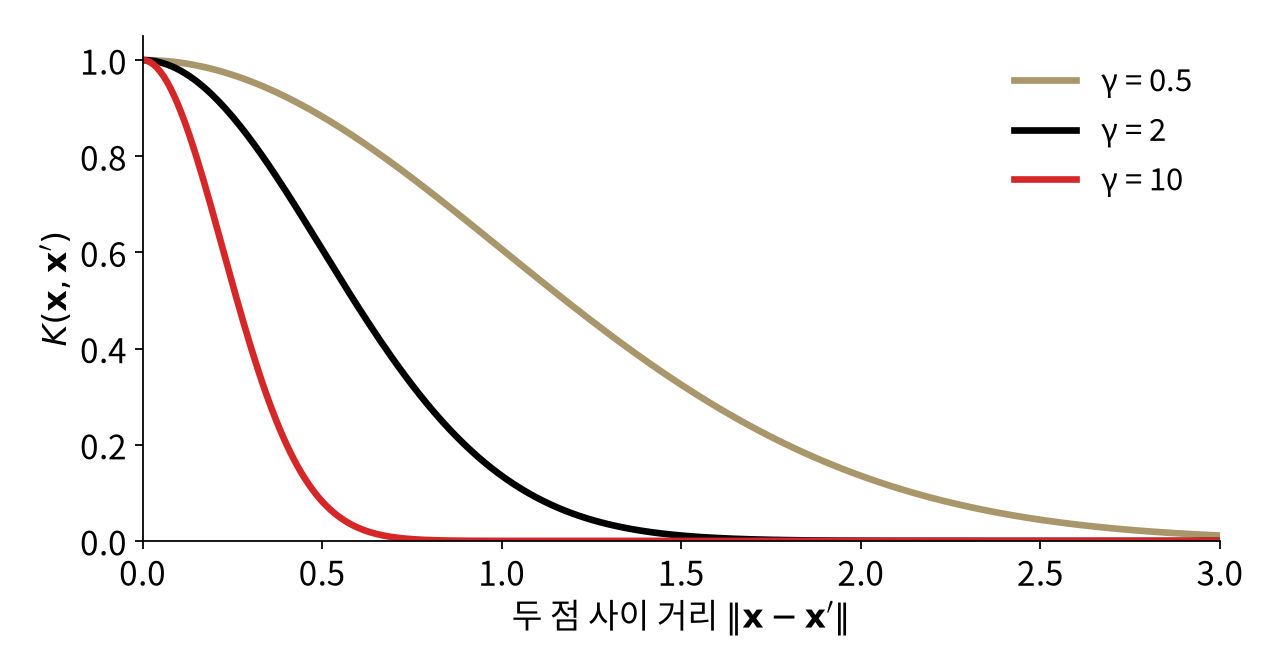
\includegraphics[width=0.62\linewidth]{sv_rbf.png}\par\vskip0.2em
{\large $K(\mathbf{x}, \mathbf{x}') = e^{-\gamma\lVert\mathbf{x}-\mathbf{x}'\rVert^2}$: 두 점이 같으면 \kb{1}, 멀면 \kb{0}}\\[0.3em]
{\normalsize $\gamma$ 가 크면 조금만 멀어져도 0 \quad ($\mathbf{x}'$ 를 중심으로 한 \kb{언덕} 하나)}
\vfill
\note{RBF 커널을 자세히 봅시다. RBF 커널은 두 점 사이 거리의 제곱에 마이너스 감마를 곱해 e의 지수로 올린 것입니다. 같은 점이면 거리가 0이라 1, 멀어질수록 0으로 떨어지는 가까움 점수입니다. 감마가 크면 조금만 멀어져도 금방 0이 되고, 작으면 멀리까지 1에 가깝게 남습니다. 대략 1 나누기 루트 감마 정도의 거리까지 영향이 미친다고 보면 됩니다. 한 점 x 프라임을 고정하고 x를 움직이면, x 프라임 자리에서 1로 가장 높고 멀어질수록 0으로 내려가는 종 모양 언덕 하나가 됩니다. 다음 쪽부터 이 언덕으로 분류기를 만듭니다.}
\end{frame}

% --- 언덕 1개 vs 서포트 벡터마다 언덕
\begin{frame}{RBF 는 $(x_1, x_2, \text{높이 하나})$ 가 아니다}
\vfill
\centering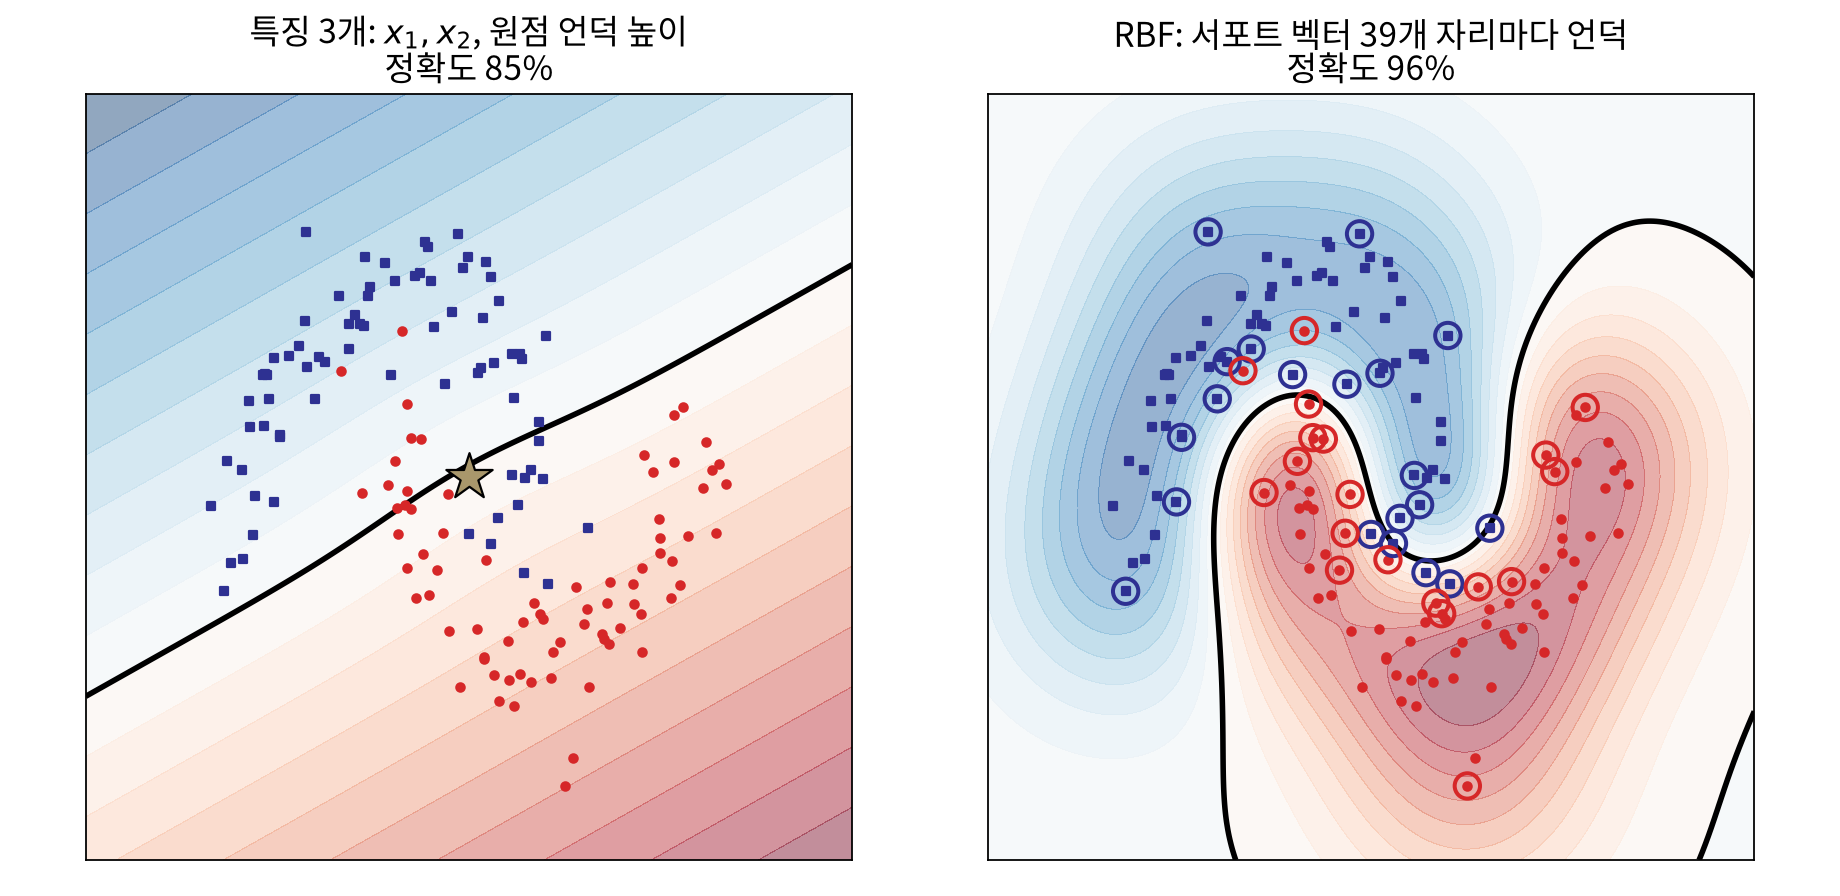
\includegraphics[width=0.72\linewidth]{sv_hills.png}\par\vskip0.2em
{\large 언덕 1개 $\to$ \kq{원 비슷한 경계만} \quad 서포트 벡터마다 언덕 (빨강 $+$, 파랑 $-$) $\to$ \kb{어떤 모양이든}}
\vfill
\note{헷갈리기 쉬운 부분입니다. 앞에서 원 모양 데이터에 높이 x1 제곱 더하기 x2 제곱을 붙여 특징 3개로 만들었습니다. 그러면 RBF도 x1, x2에 rbf 값 하나를 붙인 특징 3개일까요? 아닙니다. rbf는 점 하나로는 계산이 안 되고 기준점이 하나 더 필요합니다. 기준점을 원점 하나로 잡으면 원점에 세운 언덕 하나이고, 이것은 높이 x1 제곱 더하기 x2 제곱을 붙인 것과 같은 생각입니다. 왼쪽 그림이 반달 데이터에 그렇게 한 것입니다. 금색 별이 언덕의 중심입니다. 언덕 하나로 만들 수 있는 경계는 원 비슷한 모양뿐이라 85퍼센트에 그칩니다. RBF SVM은 오른쪽처럼 서포트 벡터마다, 동그라미 친 점마다 그 자리에 언덕을 하나씩 세우고, 빨간 서포트 벡터는 위로, 파란 서포트 벡터는 아래로 알파만큼 키워서 더합니다. 이 합이 배경색이고, 0인 곳이 검은 경계입니다. 언덕 39개를 겹치니 반달처럼 휘어진 경계도 만들어 96퍼센트를 맞힙니다. 감마는 1, C는 1입니다.}
\end{frame}

% --- RBF 피처 수
\begin{frame}{RBF 는 실제로 어떻게 계산하나: 학습 점마다 언덕 하나}
\vfill
\centering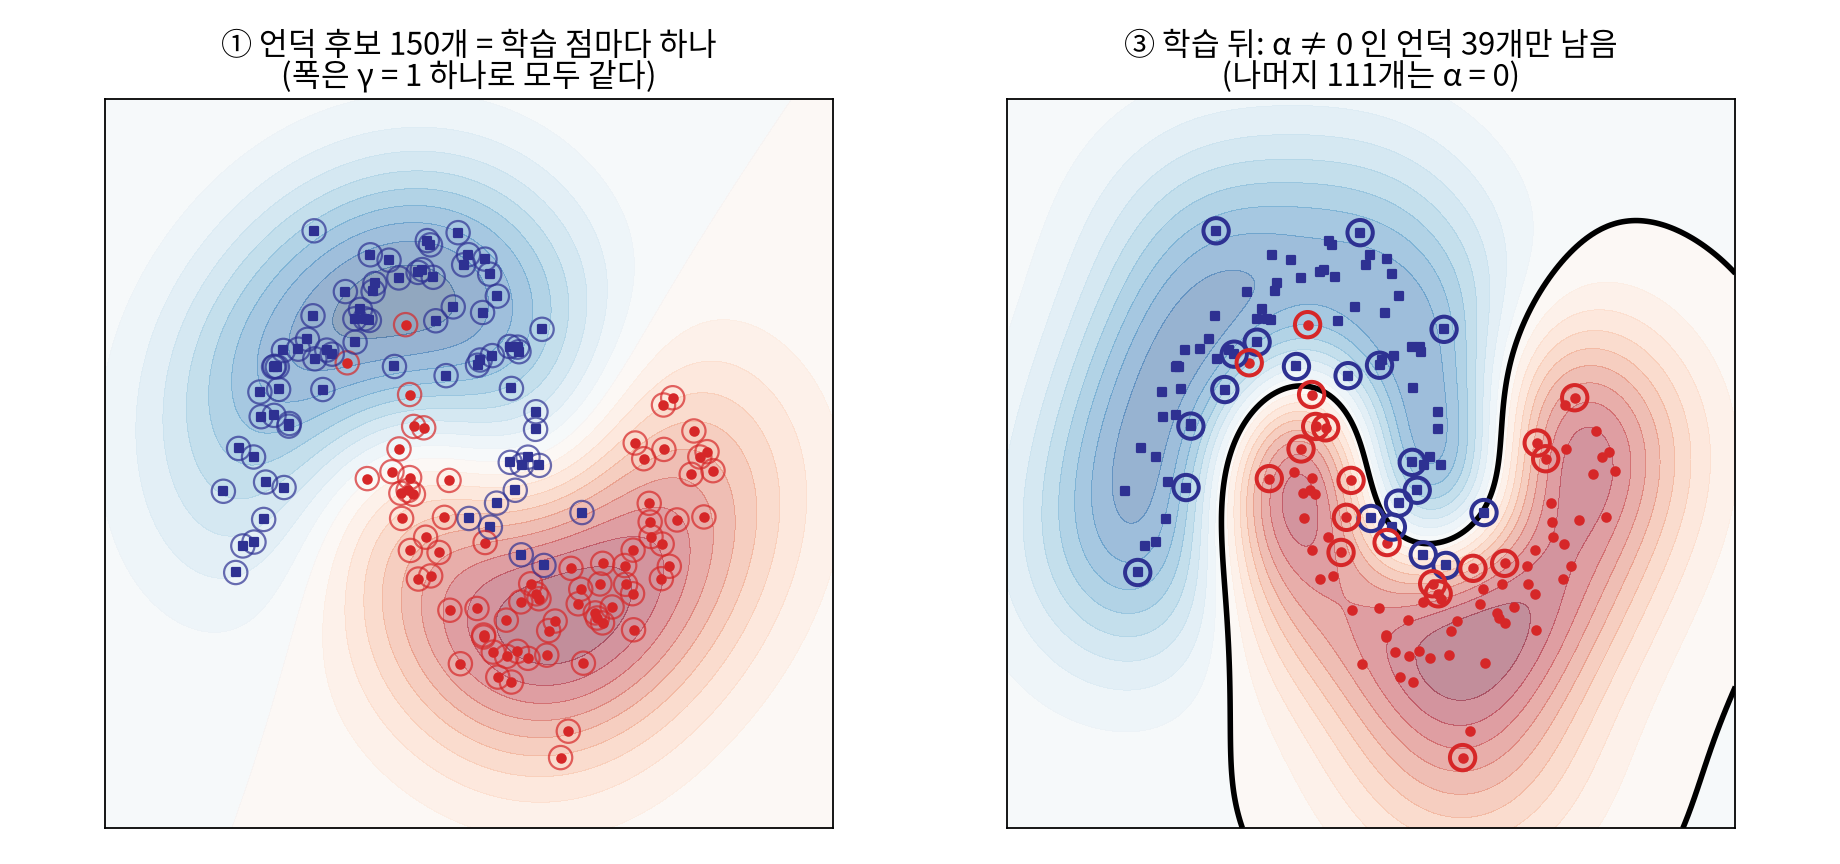
\includegraphics[width=0.56\linewidth]{sv_hill_count.png}\par\vskip0.3em
\renewcommand{\arraystretch}{1.25}
{\small\begin{tabular}{rl|rl}
\textbf{①} & 언덕 후보 = 점마다 1개 ($p = 150$), 폭 \kq{$\gamma$ 하나} &
\textbf{③} & 학습 = 높이 $\alpha_k$, 대부분 0 $\to$ \kb{39개} 남음\\
\textbf{②} & 새 점에서 언덕 150개 높이 $K(\mathbf{x}, \mathbf{x}_k)$ &
\textbf{④} & 예측 = $D(\mathbf{x}) = b + \sum_k \alpha_k y_k K$ 의 부호
\end{tabular}}\\[0.5em]
{\large 학습할 때: 언덕 후보 \kb{150개} (모든 학습 점) 다 본다 \quad 예측할 때: $\alpha_k \ne 0$ 인 \kb{39개}만 쓴다}
\vfill
\note{그러면 특징이 무한 개인 RBF를 실제로는 어떻게 계산할까요. 감마를 여러 개 쓰는 게 아닙니다. 감마는 하나이고, 학습 점마다 언덕을 하나씩 세웁니다. 단계별로 보겠습니다. 첫째, 반달 데이터는 점이 150개입니다. 점마다 그 자리를 중심으로 언덕을 하나씩 세워, 언덕 후보가 150개입니다. 중심은 다 다르고, 폭은 감마 하나로 모두 같습니다. 왼쪽 그림이 150개 언덕을 모두 같은 높이로 세운 것입니다. 둘째, 새 점 x가 오면 150개 언덕 각각에서 높이를 읽습니다. 어떤 학습 점 바로 옆이면 그 언덕 값은 1에 가깝고, 멀면 0입니다. 무한 개의 특징을 직접 만드는 대신, 학습 점 하나하나와 얼마나 가까운가, 이 150개 값으로 계산합니다. 셋째, 학습은 언덕마다 높이 알파를 정하는 것입니다. 빨간 점의 언덕은 위로, 파란 점의 언덕은 아래로입니다. SVM은 경계 근처 점만 알파가 0이 아니고, 나머지 111개는 알파가 0이 되어 언덕이 사라집니다. 남은 39개가 서포트 벡터이고, 오른쪽 그림이 그 39개 언덕을 알파만큼 키워 더한 것입니다. 넷째, 예측은 그 합 D의 부호이고, 0인 곳이 검은 경계입니다. 정리하면, 학습할 때는 150개 학습 점 모두를 언덕 후보로 놓고 알파를 정하고, 예측할 때는 알파가 0이 아닌 39개, 서포트 벡터의 언덕만 씁니다. 150개와 39개는 같은 이야기의 학습 전과 학습 후입니다. 감마는 특징 수가 아니라 언덕 폭입니다. 작으면 넓은 언덕이라 멀리까지 영향을 주어 경계가 매끈하고, 크면 좁은 언덕이라 점마다 섬이 생겨 과대적합됩니다. 감마는 학습으로 정하지 않고 교차 검증으로 하나 고릅니다. 이 150개 언덕 특징으로 로지스틱 회귀를 해도 비슷한 경계가 나오는데, SVM은 대부분의 알파를 0으로 만들어 언덕 몇 개만 남긴다는 점이 다릅니다.}
\end{frame}

% --- 참고: RBF 를 테일러 급수로 펼치기
\begin{frame}{참고: RBF 를 테일러 급수로 펼치면 다항 커널의 합}
\markpage{taylor}
\vfill
\renewcommand{\arraystretch}{1.55}
{\normalsize\begin{tabular}{rl}
\textbf{1.} & 거리 제곱 풀기: \; $\lVert\mathbf{x}-\mathbf{x}'\rVert^2 = \lVert\mathbf{x}\rVert^2 + \lVert\mathbf{x}'\rVert^2 - 2\,\mathbf{x}\cdot\mathbf{x}'$\\
\textbf{2.} & 세 개의 곱: \; $e^{-\gamma\lVert\mathbf{x}-\mathbf{x}'\rVert^2} = \underbrace{e^{-\gamma\lVert\mathbf{x}\rVert^2}\, e^{-\gamma\lVert\mathbf{x}'\rVert^2}}_{\text{각 점만의 수}}\; e^{\,2\gamma\,\mathbf{x}\cdot\mathbf{x}'}$\\
\textbf{3.} & 테일러 급수: \; $e^t = 1 + t + \dfrac{t^2}{2!} + \dfrac{t^3}{3!} + \cdots$ \quad (모든 $t$ 에서 정확히 같다)\\
\textbf{4.} & $t = 2\gamma\,\mathbf{x}\cdot\mathbf{x}'$: \; $e^{\,2\gamma\,\mathbf{x}\cdot\mathbf{x}'} = 1 + 2\gamma\,(\mathbf{x}\cdot\mathbf{x}') + \dfrac{(2\gamma)^2}{2!}(\mathbf{x}\cdot\mathbf{x}')^2 + \dfrac{(2\gamma)^3}{3!}(\mathbf{x}\cdot\mathbf{x}')^3 + \cdots$\\
 & $(\mathbf{x}\cdot\mathbf{x}')^q$ = \kb{$q$ 차 다항 커널}, \; 무게 $\dfrac{(2\gamma)^q}{q!}$ 는 차수가 높을수록 작다
\end{tabular}}\\[0.6em]
\centering
{\small 예 ($x = 1$, $x' = 0.5$, $\gamma = 1$): 항을 더하면 0.29 $\to$ 0.57 $\to$ 0.72 $\to$ 0.76 $\to$ 0.78 $= e^{-0.25}$}\\[0.3em]
{\normalsize $\gamma$ 작으면 높은 차수 무게가 금방 0 $\to$ \kb{낮은 차수 다항처럼} 매끈, \; $\gamma$ 크면 \kq{높은 차수까지} $\to$ 구불구불}\\[0.3em]
{\small 모든 차수 항을 다 세면 \kq{무한 개} $\to$ 직접 못 만든다 $\to$ SVM 은 언덕 $p$ 개로 \kb{같은} $D(\mathbf{x})$ 계산}
\vfill
\note{앞 쪽에서 RBF가 모든 차수 다항 커널의 합이라고 했는데, 그 과정을 천천히 봅시다. 첫째, 거리 제곱을 풀면 x 길이 제곱 더하기 x 프라임 길이 제곱 빼기 2 x 점곱 x 프라임입니다. 둘째, 지수의 덧셈은 곱셈으로 나뉘니까, RBF는 x에만 관한 수, x 프라임에만 관한 수, 그리고 e의 2감마 x 점곱 x 프라임 승, 세 개의 곱입니다. 앞의 두 개는 점 하나씩만의 숫자라 크기만 조절합니다. 셋째, 테일러 급수입니다. e의 t승은 1 더하기 t 더하기 t 제곱 나누기 2 팩토리얼 더하기 t 세제곱 나누기 3 팩토리얼, 이렇게 끝없이 이어지는 다항식과 모든 t에서 정확히 같습니다. 넷째, t 자리에 2감마 x 점곱 x 프라임을 넣으면 점곱의 0제곱, 1제곱, 2제곱, 3제곱이 차례로 나옵니다. 점곱의 q제곱은 바로 q차 다항 커널이고, 앞에 붙는 무게 2감마의 q제곱 나누기 q 팩토리얼은 q가 커질수록 팩토리얼 때문에 금방 작아집니다. 그래서 RBF는 1차, 2차, 3차, 끝없이 모든 차수의 다항 커널을 높은 차수일수록 작은 무게로 다 더한 것이고, 특징으로 쓰면 무한 차원입니다. 아래는 1차원 숫자 예입니다. x가 1, x 프라임이 0.5, 감마가 1이면 정확한 값은 e의 마이너스 0.25승, 0.78입니다. 앞의 두 수를 곱한 0.29에서 시작해 항을 하나씩 더하면 0.57, 0.72, 0.76, 0.78로 정확한 값에 다가갑니다. 다섯 항 정도면 거의 같아집니다. 그래서 RBF는 다항 커널과 친척입니다. 감마가 무게를 정하는데, 감마가 작으면 2감마의 q제곱이 아주 작아서 높은 차수 항은 거의 0이고, 1차, 2차 정도만 남아 낮은 차수 다항 커널처럼 매끈한 경계가 됩니다. 감마가 크면 높은 차수 항까지 무게가 살아 있어 아주 높은 차수 다항식처럼 구불구불한 경계가 됩니다. 다음 쪽 감마 그림이 바로 이것입니다. 다만 정확히 같지는 않습니다. 앞의 두 수, 각 점의 길이에 따른 수가 곱해지고 차수가 끝없이 이어지니, 거리로 재는 유사도라는 성질은 RBF만의 것입니다. 그리고 실용적인 장점이 하나 있습니다. 다항 커널은 차수 q를 몇으로 할지 골라야 하는데, RBF는 모든 차수가 이미 들어 있고 감마가 무게를 낮은 차수 쪽이나 높은 차수 쪽으로 옮겨 줍니다. 그래서 차수를 따로 고를 필요 없이 감마 하나만, C와 함께 교차 검증으로 고르면 됩니다. RBF가 기본 커널로 많이 쓰이는 이유 중 하나입니다. 실제로 sklearn의 SVC도 기본 커널이 RBF입니다.}
\end{frame}

% --- 참고: γ 에 따라 닮는 차수
\begin{frame}{참고: $\gamma$ 에 따라 몇 차 다항과 닮나}
\vfill
\centering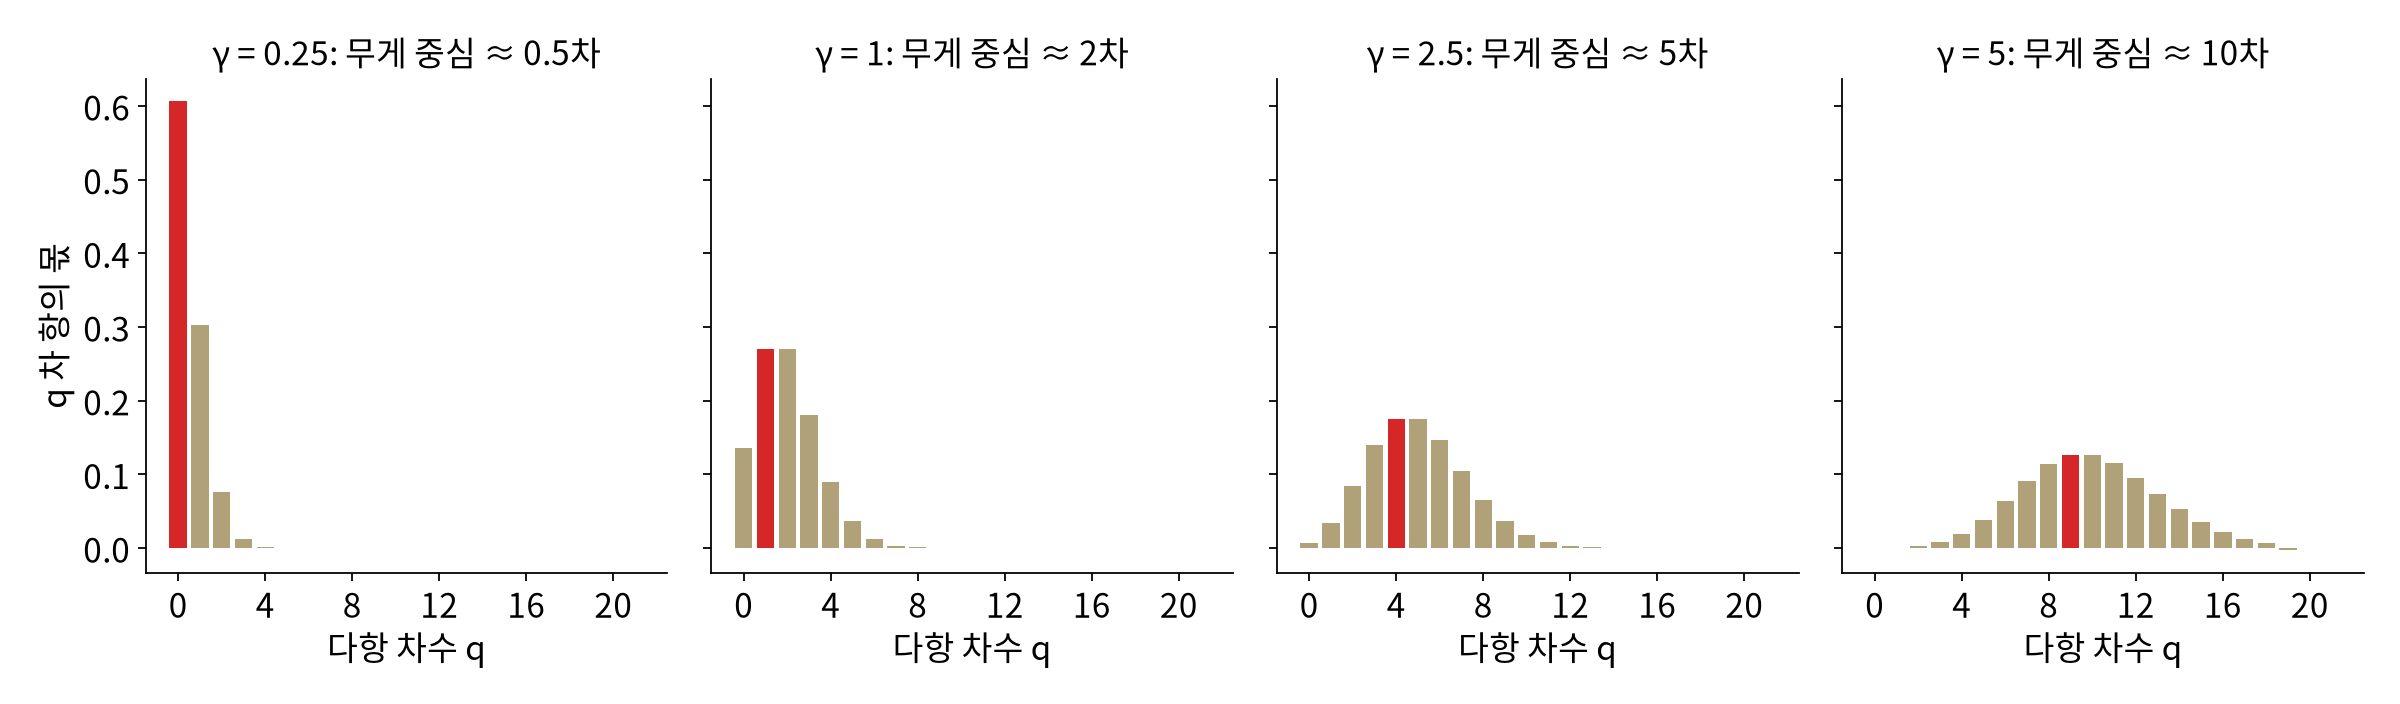
\includegraphics[width=0.96\linewidth]{sv_rbf_degree.png}\par\vskip0.3em
{\large $\mathbf{x}\cdot\mathbf{x}' = 1$ 일 때 $q$ 차 항의 몫 $\propto \dfrac{(2\gamma)^q}{q!}$ \;$\to$\; 무게 중심 $= 2\gamma$ 차}\\[0.3em]
{\normalsize $\gamma$ 를 키우면 무게가 \kq{높은 차수}로 옮겨 간다 $\to$ 구불구불한 경계 (다음 쪽)}
\vfill
\note{앞 쪽에서 RBF는 모든 차수 다항의 합이고, q차 항 앞의 무게가 2감마의 q제곱 나누기 q 팩토리얼이라고 했습니다. 그러면 감마에 따라 어느 차수에 무게가 몰리는지 그려 볼 수 있습니다. x 점곱 x 프라임이 1일 때 각 차수 항의 크기를 합이 1이 되게 나눠 막대로 그렸습니다. 빨간 막대가 가장 큰 차수입니다. 감마가 0.25면 0차와 1차가 대부분이라 거의 직선에 가깝습니다. 감마가 1이면 1차와 2차, 무게 중심이 2차라서 2차 다항 커널과 비슷합니다. 감마가 2.5면 5차 근처, 감마가 5면 10차 근처까지 무게가 옮겨 갑니다. 이 막대 모양은 평균이 2감마인 포아송 분포와 같아서, 무게 중심은 정확히 2감마 차입니다. 점곱이 1이 아니면 무게 중심은 2감마 곱하기 점곱 차로 옮겨 갑니다. 그래서 데이터를 z-score 해서 점곱이 1 근처가 되게 해 두면, 감마를 대략 몇 차 다항처럼 쓸지로 읽을 수 있습니다. 감마를 키울수록 높은 차수 다항처럼 구불구불해지는 것이 다음 쪽 그림입니다. 다만 이건 감을 잡기 위한 그림이고, 실제로는 감마를 교차 검증으로 고릅니다.}
\end{frame}

% --- gamma
\begin{frame}{RBF 커널의 $\gamma$: 얼마나 구불구불하게}
\vfill
\centering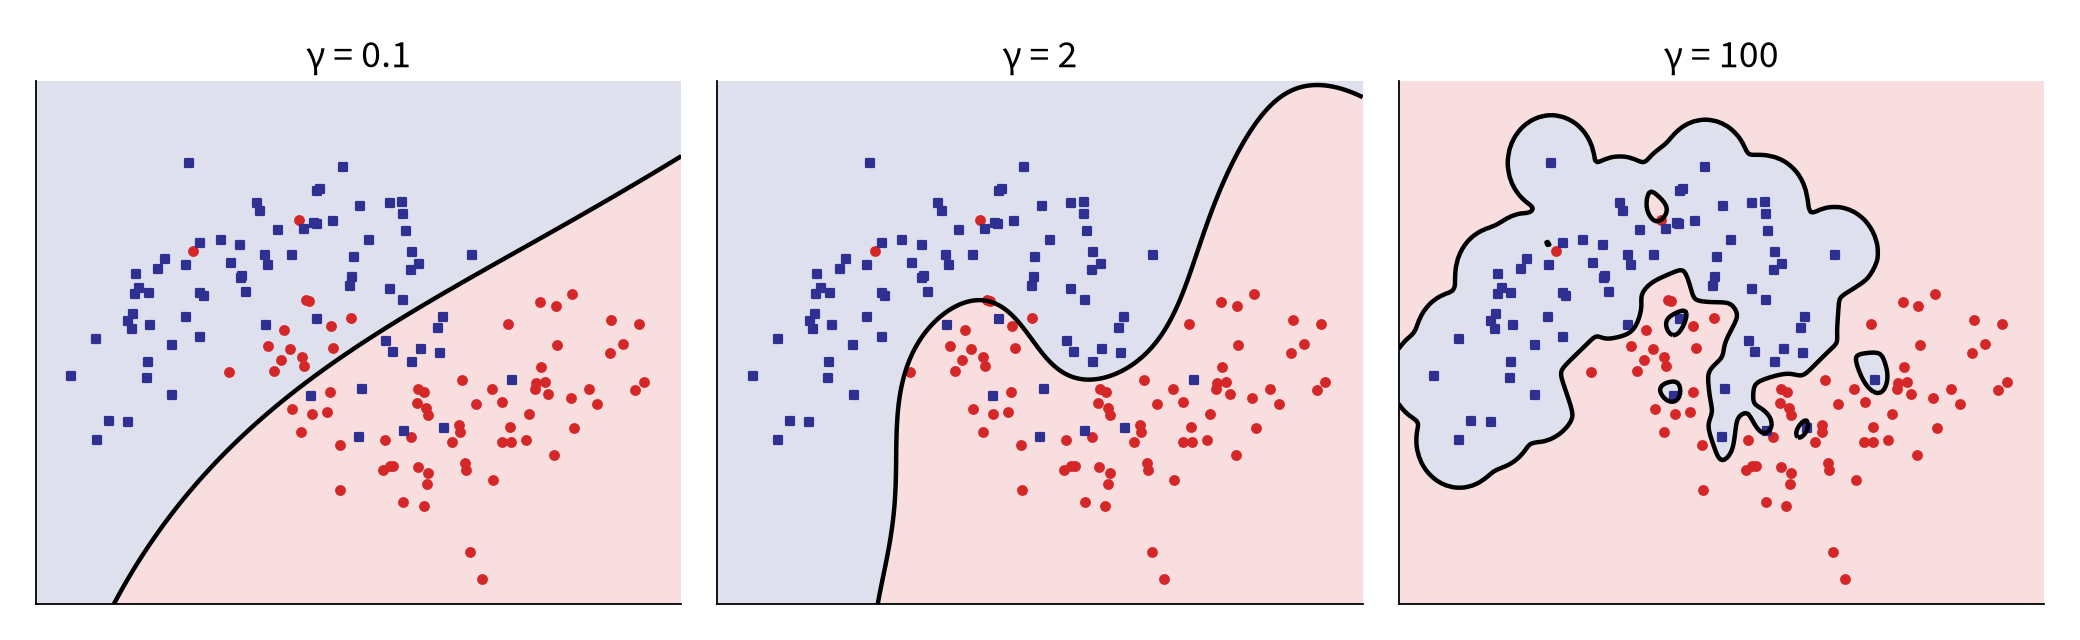
\includegraphics[width=0.92\linewidth]{sv_gamma.png}\par\vskip0.2em
{\large $\gamma$ 작으면 과소적합 \quad 크면 \kq{과대적합}}
\vfill
\note{RBF 커널의 감마는 앞 쪽의 언덕 폭, 점 하나의 영향이 얼마나 멀리까지 미치는지를 정합니다. 대략 1 나누기 루트 감마 거리까지입니다. 감마가 0.1로 작으면 영향이 넓게 퍼져서 경계가 거의 직선입니다. 반달 모양을 못 따라가는 과소적합입니다. 감마가 2면 반달을 따라 적당히 휘어집니다. 감마가 100이면 점 하나하나의 영향이 아주 좁아서 점마다 섬이 생깁니다. 학습 데이터를 외운 과대적합입니다. 그래서 SVM을 쓸 때는 C와 감마 두 숫자를 교차 검증으로 함께 고릅니다. 실습에서 직접 해 봅니다.}
\end{frame}

\section{논문 식}
% --- 논문 식 읽기 ①
\begin{frame}{논문 식 읽기 ①: 라그랑주 함수와 닿은 점}
\vfill
\centering
{\large\begin{gather*}
L(\mathbf{w}, b, \boldsymbol{\alpha}) = \tfrac{1}{2}\lVert\mathbf{w}\rVert^2 - \sum_{k=1}^{p} \alpha_k\,\big[\,y_k D(\mathbf{x}_k) - 1\,\big], \qquad \alpha_k \ge 0\\[0.3em]
\alpha_k\,\big(\,y_k D(\mathbf{x}_k) - 1\,\big) = 0
\end{gather*}}\\[0.3em]
{\large 곱이 0 $\to$ 가장자리에 \kq{안 닿은} 점 (값 $> 1$) 은 $\alpha_k = 0$}\\[0.5em]
{\normalsize 이 데이터: 서포트 벡터 3개만 값 $= 1$ $\to$ $\alpha = 1.1$ · $0.55$ · $0.55$, \;나머지 17개는 값 $\ge 1.21$ $\to$ $\alpha = 0$}
\vfill
\note{지금까지 배운 것을 원 논문의 식으로 한 번씩 읽어 봅시다. 첫 식은 논문 식 14, 라그랑주 함수입니다. 2분의 1 w 길이 제곱을 줄이고 싶은데, 모든 점의 값이 1 이상이어야 한다는 조건이 붙어 있습니다. 라그랑주 방법은 조건마다 숫자 하나, 알파 k를 붙여서 조건을 식 안으로 넣습니다. 대괄호 안, y k D x k 빼기 1은 점 k가 조건을 얼마나 넉넉하게 지키는지입니다. 둘째 식은 논문 식 15입니다. 알파 k와 대괄호 안의 곱이 0입니다. 곱이 0이면 둘 중 하나는 0이어야 합니다. 그래서 가장자리에 닿지 않은 점, 값이 1보다 큰 점은 알파가 0이고, 알파가 0이 아닐 수 있는 점은 값이 딱 1인 점, 가장자리에 닿은 서포트 벡터뿐입니다. 역학 비유에서 닿아 있을 때만 힘이 생긴다고 한 것이 이 식입니다. 이 데이터에서 확인하면, 서포트 벡터 3개는 값이 1이고 알파가 1.1, 0.55, 0.55입니다. 나머지 17개는 값이 1.21 이상이라 알파가 0입니다.}
\end{frame}

% --- 논문 식 읽기 ②
\begin{frame}{논문 식 읽기 ②: 미분하면 $\mathbf{w}$, $\mathbf{w}$ 를 지우면 $K$ 만}
\vfill
\centering
{\large\begin{gather*}
\frac{\partial L}{\partial \mathbf{w}} = \mathbf{w} - \sum_{k} \alpha_k y_k \mathbf{x}_k = 0 \quad\to\quad \mathbf{w}^* = \sum_{k} \alpha_k y_k \mathbf{x}_k\\[0.3em]
J(\boldsymbol{\alpha}, b) = \sum_{k} \alpha_k\,(1 - b\,y_k) - \tfrac{1}{2}\sum_{k}\sum_{l} \alpha_k \alpha_l\, y_k y_l\, K(\mathbf{x}_k, \mathbf{x}_l)
\end{gather*}}\\[0.3em]
{\large $\mathbf{w}$ 가 사라지고 점은 \kb{$K$ 안에만} $\to$ 커널로 학습}\\[0.5em]
{\normalsize 이 데이터: $\mathbf{w}^* = 1.1\,r - 0.55\,b_1 - 0.55\,b_2 = (1.05,\ 1.05)$}
\vfill
\note{다음은 논문 식 16과 17입니다. 라그랑주 함수 L을 w로 미분해서 0으로 두면, w 빼기 알파 k y k x k의 합이 0, 즉 w 별은 알파 k y k x k의 합입니다. 덱에서 학습을 알파로 다시 쓰며 본 바로 그 식이 미분 한 번으로 나옵니다. 커널을 쓰면 x k 자리가 파이 x k입니다. 이 w를 다시 L에 넣으면 w가 사라지고 알파와 b만 남는 J가 됩니다. 앞의 합은 알파 k 곱하기 1 빼기 b y k이고, 뒤는 알파끼리, 라벨끼리 곱하고 두 점의 K를 곱한 것의 합의 절반입니다. 논문은 뒤의 항을 알파 점 H 점 알파로 쓰고, H k l이 y k y l K x k x l인 행렬이라고 적습니다. 중요한 것은 점이 들어가는 곳이 K 하나뿐이라는 것입니다. 그래서 학습에도 파이를 만들 필요가 없고, 커널 SVM 학습에서 학습 점 두 개를 넣은 K 값만 계산한다고 했던 것이 이 식입니다. 이 데이터에서는 w 별이 1.1 r 빼기 0.55 b1 빼기 0.55 b2, 1.05, 1.05입니다.}
\end{frame}

% --- 논문 식 읽기 ③
\begin{frame}{논문 식 읽기 ③: 분류기, $b$, 마진}
\vfill
\centering
{\large\begin{align*}
D(\mathbf{x}) &= \sum_{k} y_k \alpha_k^*\, K(\mathbf{x}_k, \mathbf{x}) + b\\[0.2em]
b^* &= -\tfrac{1}{2}\,\big(\mathbf{w}^*\cdot\mathbf{x}_A + \mathbf{w}^*\cdot\mathbf{x}_B\big) \qquad (\mathbf{x}_A, \mathbf{x}_B:\ \text{빨강 · 파랑 서포트 벡터 하나씩})\\[0.2em]
\tfrac{1}{2}\lVert\mathbf{w}^*\rVert^2 &= \frac{1}{2M^2} = \tfrac{1}{2}\sum_{k} \alpha_k^*
\end{align*}}\\[0.3em]
{\normalsize 이 데이터: \; $b^* = -\tfrac12(0.95 - 1.05) = 0.05$, \quad $\lVert\mathbf{w}^*\rVert^2 = 2.2 = 1/0.67^2 = 1.1 + 0.55 + 0.55$}
\vfill
\note{논문 식 18, 19, 20입니다. 첫 줄은 학습이 끝난 분류기로, 앞에서 쓴 D x와 같습니다. 서포트 벡터마다 y 곱하기 알파 곱하기 K를 더하고 b를 더합니다. 둘째 줄은 b를 정하는 식입니다. 경계는 두 클래스의 한가운데라, 빨강 서포트 벡터 하나는 값이 플러스 1, 파랑 하나는 마이너스 1입니다. 두 값의 평균이 0이 되게 b를 정하면 b 별은 마이너스 2분의 1 곱하기 두 점의 w 점곱의 합입니다. 이 데이터에서 빨강 r은 w 점곱이 0.95, 파랑 b1은 마이너스 1.05이니, 마이너스 2분의 1 곱하기 마이너스 0.1, 0.05입니다. 셋째 줄은 마진과 알파의 관계입니다. 가장 가까운 값을 1로 두었으니 마진은 1 나누기 w의 길이이고, 그래서 w 길이 제곱은 1 나누기 M 제곱입니다. 그리고 그것이 알파를 다 더한 것과 같습니다. 이 데이터에서 w 길이 제곱은 2.2, 1 나누기 0.67의 제곱도 2.2, 알파의 합 1.1 더하기 0.55 더하기 0.55도 2.2입니다. 마진이 좁을수록 알파가 커지니, 길을 좁게 받치는 점일수록 세게 민다는 뜻입니다. 논문은 이 식으로 알파가 가장 큰 점을 빼면 마진이 가장 많이 넓어진다고 하고, 그 점을 이상치로 찾아냅니다.}
\end{frame}

% --- 논문 식 읽기 ④
\begin{frame}{논문 식 읽기 ④: 실험, 특징 수가 폭발해도 서포트 벡터는 그대로}
\vfill
\centering
{\large 다항 커널 $K(\mathbf{x}, \mathbf{x}') = (\mathbf{x}\cdot\mathbf{x}' + 1)^q$ \;· 손글씨 숫자 16 $\times$ 16 ($n = 256$)}\\[0.6em]
\renewcommand{\arraystretch}{1.3}
{\large\begin{tabular}{c|r|r|r}
차수 $q$ & 특징 수 $N$ & 시험 오류 & 서포트 벡터 수\\ \hline
1 & 256 & 10.5\% & 97\\
2 & $3 \times 10^4$ & 5.8\% & 89\\
3 & $8 \times 10^7$ & 5.2\% & 79\\
4 & $4 \times 10^9$ & \kb{4.9\%} & 72\\
5 & $1 \times 10^{12}$ & 5.2\% & 69
\end{tabular}}\\[0.6em]
{\normalsize $N$ 은 1조 개까지 늘어도 실제로 쓰는 건 서포트 벡터 \kb{70개 남짓}}\\[0.2em]
{\normalsize 차수를 부드럽게 바꾸는 커널도: \;$K(\mathbf{x}, \mathbf{x}') = e^{\gamma\,\mathbf{x}\cdot\mathbf{x}'} - 1$}
\vfill
\note{마지막은 논문의 실험입니다. 미국 우편물에서 모은 16 곱하기 16 픽셀 손글씨 숫자로, 원래 특징은 256개입니다. 다항 커널 x 점곱 x 프라임 더하기 1의 q제곱으로 차수를 1부터 5까지 올렸습니다. 특징 수 N은 256에서 3만, 8천만, 40억, 1조로 폭발합니다. 그런데 숫자 하나를 가르는 경계마다 쓰인 서포트 벡터는 평균 97개에서 69개로 오히려 줄고, 시험 오류는 10.5퍼센트에서 4차일 때 4.9퍼센트까지 내려갑니다. 특징을 직접 1조 개 만들었다면 불가능했을 학습을 커널로 했다는 증거이고, 특징 수가 아니라 서포트 벡터 수가 모델의 복잡도를 정한다는 논문의 주장을 보여 줍니다. 4.9퍼센트는 같은 데이터에서 LeCun 등의 5층 신경망이 낸 5.1퍼센트보다 조금 낫습니다. 논문은 차수를 1, 2, 3처럼 계단으로만 올리지 말고 부드럽게 조절하려고 식 21, e의 감마 x 점곱 x 프라임 승 빼기 1이라는 커널도 씁니다. e의 지수를 펼치면 모든 차수 다항의 합이라, RBF 테일러 쪽에서 본 것처럼 감마가 작으면 낮은 차수, 크면 높은 차수처럼 움직입니다. 다른 데이터에서 감마 0.75일 때 오류 1.3퍼센트였습니다.}
\end{frame}

\section{정리}
% --- 장단점
\begin{frame}{SVM 정리: 장점과 단점}
\vfill
\centering
\renewcommand{\arraystretch}{1.6}
{\large\begin{tabular}{c|c}
{\Large\kb{장점}} & {\Large\kq{단점}}\\ \hline
볼록 최적화 $\to$ 답이 \textbf{하나} & $C$ · 커널 · $\gamma$ 를 골라야 한다 (교차 검증)\\
$C$ 로 과대적합 조절 & 기본은 \textbf{두 클래스}용\\
커널로 경계 모양이 자유롭다 & 해석이 어렵다, 확률을 주지 않는다\\
예측엔 서포트 벡터만 필요 & 데이터가 아주 많으면 학습이 느리다
\end{tabular}}
\vfill
\note{정리하면 SVM의 장점은 첫째, 볼록 최적화 문제라 답이 하나로 정해지고 시작점에 따라 달라지지 않습니다. 둘째, C로 과대적합을 조절할 수 있습니다. 셋째, 커널을 바꿔 경계 모양을 자유롭게 만들 수 있습니다. 넷째, 예측할 때 서포트 벡터만 있으면 됩니다. 단점은 C, 커널, 감마 같은 숫자를 교차 검증으로 골라야 하고, 기본적으로 두 클래스를 가르는 방법이며, 로지스틱회귀처럼 확률을 주지 않고 왜 그렇게 분류했는지 해석하기 어렵다는 점입니다. 데이터가 많으면 커널 SVM의 학습이 느려지는 것도 단점입니다. 이유는 커널이 두 점씩 짝으로 계산되기 때문입니다. 학습할 때는 원칙적으로 모든 짝의 K가 필요해서, 점이 1만 개면 1만 곱하기 1만, 1억 개이고 다 저장하면 약 800메가바이트입니다. sklearn은 이 표를 한꺼번에 만들지 않고 두 점씩 고쳐 가며 필요한 줄만 그때그때 계산하지만, 그래도 학습 시간이 점 수의 제곱 이상으로 늘어 수만 개를 넘으면 현실적이지 않습니다. 예측할 때는 서포트 벡터만 쓰니 그 수만큼만 K를 계산합니다. 데이터가 크면 커널 없는 선형 SVM을 쓰거나, RBF 특징을 수백 개로 근사해 만드는 방법, 예를 들어 sklearn의 Nystroem이나 RBFSampler를 쓰거나, 트리 부스팅이나 신경망 같은 다른 모델을 씁니다. RBF SVM이 잘 맞는 것은 실습의 지폐 데이터 1,372개처럼 수천에서 수만 개 정도의 데이터입니다.}
\end{frame}

\section{연습}
% --- 실습
\begin{frame}{실습}
\vfill
\centering\begin{tabular}{rl}
\large 1 & 원 데이터: 특징 6개 직접 만들기 (A) vs 다항 커널 (B) 가 같은 $\mathbf{w}$ 인지 확인\\[0.5em]
\large 2 & 실제 데이터: 지폐 1,372장 진위 판별, 선형 vs RBF\\[0.5em]
\large 3 & 반달 데이터에서 $C$ 와 $\gamma$ 를 교차 검증으로 고르기
\end{tabular}\vskip1em
Banknote Authentication (Lohweg; UCI) \\[0.4em]\href{https://colab.research.google.com/github/SuminHan/book-ml/blob/main/slides/ml1/week02/3_svm_kernel/lab/svm_kernel.ipynb}{\textcolor{ksagolddk}{▶ Colab에서 실습 노트북 열기}}
\vfill
\note{실습은 세 부분입니다. 첫째, 원 데이터에서 특징 6개를 직접 만들어 선형 SVM으로 학습한 w와, 다항 커널로 학습한 알파로 계산한 w가 같은지 확인합니다. 둘째, 지폐 사진에서 뽑은 특징 4개로 진짜 지폐와 위조지폐를 가리는 실제 데이터에서 선형 SVM과 RBF SVM을 비교합니다. 셋째, 반달 데이터에서 sklearn의 C와 감마를 교차 검증으로 고르고 경계를 그려 봅니다. sklearn의 C는 지난 시간의 C와 같아서, 크면 좁은 길입니다.}
\end{frame}

% --- 정리
\begin{frame}{정리}
\vfill
\centering\normalsize\begin{tabular}{l}
\textbf{특징 늘리기}: 점에 숫자를 붙여 올리면, 올린 곳의 직선 = 원래 자리의 \kb{휘어진 경계}\\[0.5em]
\textbf{커널}: $K(\mathbf{x}, \mathbf{x}') = \varphi(\mathbf{x})\cdot\varphi(\mathbf{x}')$ 를 $\varphi$ 없이 바로 계산\\[0.5em]
\textbf{두 방법}: A 특징 직접 $\to$ $\mathbf{w}$ (특징마다) \;=\; B 커널 $\to$ $\alpha$ (점마다), \;$\mathbf{w} = \sum_k \alpha_k y_k \varphi(\mathbf{x}_k)$\\[0.5em]
\textbf{특징 수}: 선형 2 · 다항 2차 6 · RBF $\infty$ (그래서 RBF 는 커널로만)\\[0.5em]
\textbf{RBF}: 학습 점마다 언덕, 폭 $\gamma$ 하나, 예측엔 서포트 벡터의 언덕만\\[0.5em]
\textbf{$\gamma$}: 작으면 매끈 (과소적합), 크면 구불구불 (\kq{과대적합}) $\to$ 교차 검증
\end{tabular}\par\vskip0.6em
{\tiny\color{gray} 구성 참고: S. Wang, CME 250 Lecture 5: Support Vector Machines (Stanford, Winter 2019), \href{https://web.stanford.edu/class/cme250/files/cme250_lecture5.pdf}{\textcolor{ksagolddk}{web.stanford.edu/class/cme250/files/cme250\_lecture5.pdf}} · James et al., \textit{An Introduction to Statistical Learning}, 9장\\ 원 논문: Boser, Guyon, Vapnik (1992), A training algorithm for optimal margin classifiers, COLT (커널 · RBF) · Cortes, Vapnik (1995), Support-vector networks, \textit{Machine Learning} 20(3) (소프트 마진) · Burges (1998), A tutorial on support vector machines for pattern recognition (역학 비유)}
\vfill
\note{정리합니다. 점에 숫자, 즉 특징을 붙여 높은 차원으로 올리면, 올린 곳에서 직선으로 가르는 것이 원래 자리에서는 휘어진 경계가 됩니다. 커널은 올린 뒤의 점곱을, 올리지 않고 원래 점으로 바로 계산하는 함수입니다. 같은 경계를 만드는 방법이 둘인데, 특징을 직접 만들어 특징마다 w를 학습하는 것과, 커널로 점마다 알파를 학습하는 것이고, w는 알파 곱하기 y 곱하기 파이의 합이라 둘은 같은 경계입니다. 특징 수는 선형 2, 다항 2차 6, RBF는 무한이라 RBF는 커널로만 계산합니다. RBF는 학습 점마다 언덕을 세우고 폭은 감마 하나이며, 예측할 때는 서포트 벡터의 언덕만 씁니다. 감마가 작으면 매끈하고 크면 구불구불해서 과대적합되니 교차 검증으로 고릅니다.}
\end{frame}
\end{document}
